\documentclass[tese,capa]{texufpel}

\usepackage{madsantos}
\usepackage[utf8]{inputenc}

% \usepackage{tocbibind}
% \usepackage{tocloft}
% \usepackage{xpatch}

% \newcommand{\listequationsname}{List of Equations}
% \newlistof{myequations}{equ}{\listequationsname}
% \newcommand{\myequations}[1]{%
% \addcontentsline{equ}{myequations}{\protect\numberline{\theequation}#1}}

% \xpretocmd{\listofmyequations}{\addcontentsline{toc}{chapter}{\listequationsname}}{}{}

% %% aspas: ``crase''
%%%%% BEGIN: UPS, UPSOK, TALVEZ, TIRAR e TROCAR
\usepackage{xargs}
\usepackage[textsize=tiny]{todonotes}
\usepackage[normalem]{ulem}
\usepackage{xcolor}
%\usepackage[textwidth=1.35cm,colorinlistoftodos,prependcaption,textsize=tiny]{todonotes}
\newcommandx{\trocar}[2]{{\textcolor{red}{\sout{#1}}}{{\textcolor{blue}{\textrm{#2}}}}}
\newcommandx{\talvez}[2]{{\textcolor{red}{#1}}{{\textcolor{green}{\textrm{(#2?)}}}}}
\newcommandx{\tirar}[1]{{\textcolor{red}{\sout{#1}}}}
\newcommandx{\inserir}[1]{{\textcolor{green}{#1}}}
\newcommandx{\ups}[2][1=]{\todo[linecolor=red,backgroundcolor=red!25,bordercolor=red,#1]{#2}}
\newcommandx{\upsok}[2][1=]{\todo[linecolor=blue,backgroundcolor=blue!25,bordercolor=blue,#1]{#2}}
%%%%% END: UPS, UPSOK, TALVEZ, TIRAR e TROCAR


\unidade{Centro de Desenvolvimento Tecnológico}
\programa{Programa de Pós-Gradua\-ção em Computação}
\curso{Ciência da Computação}

\unidadeeng{Technology Development Center}
\programaeng{Postgraduate Program in Computing}
\cursoeng{Computer Science}

\title{Impactos da Adoção de Infraestruturas de Nuvem no Desenvolvimento de Pesquisas Acadêmicas}

\author{Santos}{Maicon Ança dos}
\advisor[Prof.~Dr.]{Cavalheiro}{Gerson Geraldo H.}

%Palavras-chave em PT_BR
\keyword{Palavrachave-um}
\keyword{Palavrachave-dois}
\keyword{Palavrachave-tres}
\keyword{Palavrachave-quatro}

%Palavras-chave em EN_US
\keywordeng{Keyword-one}
\keywordeng{Keyword-two}
\keywordeng{Keyword-three}
\keywordeng{Keyword-four}

\begin{document}

\maketitle 

\sloppy

\fichacatalografica

%Composição da Banca Examinadora
\begin{aprovacao}{30 de fevereiro de 2019} %data da banca por extenso
\noindent Prof. Dr. Marilton Sanchotene de Aguiar (orientador)\\
Doutor em Computação pela Universidade Federal do Rio Grande do Sul.\\[1cm]

\noindent Prof. Dr. Paulo Roberto Ferreira Jr.\\
Doutor em Computação pela Universidade Federal do Rio Grande do Sul.\\[1cm]

\noindent Prof. Dr. Ricardo Matsumura Araujo\\
Doutor em Computação pela Universidade Federal do Rio Grande do Sul.\\[1cm]

\noindent Prof. Dr. Luciano da Silva Pinto\\
Doutor em Biotecnologia pela Universidade Federal de Pelotas.
\end{aprovacao}

%Opcional
\begin{dedicatoria}
  Dedico\ldots 
\end{dedicatoria}

%Opcional
\begin{agradecimentos}
  Agradeço\ldots 
\end{agradecimentos}

%Opcional
\begin{epigrafe}
  Só sei que nada sei.\\
  {\sc --- Sócrates}
\end{epigrafe}

%Resumo em Portugues (no maximo 500 palavras)
\begin{abstract}
% Bla blabla blablabla bla.  Bla blabla blablabla bla.  Bla blabla
% blablabla bla.  Bla blabla blablabla bla.  Bla blabla blablabla bla.
% Bla blabla blablabla bla.  Bla blabla blablabla bla.  Bla blabla
% blablabla bla.  Bla blabla blablabla bla.  Bla blabla blablabla bla.
% Bla blabla blablabla bla.  Bla blabla blablabla bla.  Bla blabla
% blablabla bla.  Bla blabla blablabla bla.  Bla blabla blablabla bla.
% Bla blabla blablabla bla.  Bla blabla blablabla bla.  Bla blabla
% blablabla bla.  Bla blabla blablabla bla.  Bla blabla blablabla bla.
% Bla blabla blablabla bla.
\end{abstract}

%Resumo em Inglês (no maximo 500 palavras)
\begin{englishabstract}{Impacts of the Adoption of Cloud Infrastructures on the Development of Academic Research}
% Bla blabla blablabla bla.  Bla blabla blablabla bla.  Bla blabla
% blablabla bla.  Bla blabla blablabla bla.  Bla blabla blablabla bla.
% Bla blabla blablabla bla.  Bla blabla blablabla bla.  Bla blabla
% blablabla bla.  Bla blabla blablabla bla.  Bla blabla blablabla bla.
% Bla blabla blablabla bla.  Bla blabla blablabla bla.  Bla blabla
% blablabla bla.  Bla blabla blablabla bla.  Bla blabla blablabla bla.
% Bla blabla blablabla bla.  Bla blabla blablabla bla.  Bla blabla
% blablabla bla.  Bla blabla blablabla bla.  Bla blabla blablabla bla.
% Bla blabla blablabla bla.
\end{englishabstract}

%Lista de Figuras
\listoffigures

%Lista de Tabelas
\listoftables

\chapter*{\listabbrvname}
\acronymused{CAPEX}
\acronymused{CNPq}
\acronymused{CPU}
\acronymused{Gbps}
\acronymused{HPC}
\acronymused{IaaS}
\acronymused{IEP}
\acronymused{LGPD}
\acronymused{M}
\acronymused{MPI}
\acronymused{OE}
\acronymused{OPEX}
\acronymused{QP}
\acronymused{ROI}
\acronymused{RSL}
\acronymused{SLA}
\acronymused{TCO}
\acronymused{vCPU}

\listasiglas{_Abreviaturas}

%lista de abreviaturas e siglas
\begin{listofabbrv}{CAPEX}%coloque aqui a maior sigla para ajustar a distância
        \item[CAPEX] asdll asdas dds
        \item[\textbf{ABNT}] Associação Brasileira de Normas Técnicas
        \item[NUMA] \textit{Non-Uniform Memory Access}
        \item[SIMD] Single Instruction Multiple Data
        \item[SMP] Symmetric Multi-Processor
        \item[SPMD] Single Program Multiple Data
\end{listofabbrv}

% \clearpage
% \listofmyequations

% Lista de tarefas pendentes
\listoftodos % REMOVER NA VERSÃO FINAL

%Sumario
\tableofcontents

\chapter{Introdução}

O modelo de computação em nuvem se apresenta como uma infraestrutura de suporte à execução sob demanda para aplicações que vão desde simples portais web a grandes fluxos de trabalho científicos. Neste ambiente computacional, recursos podem ser rapidamente provisionados e liberados com o mínimo esforço de gerenciamento ou interação com o provedor de serviços \cite{mell_nist_2011}.

Uma nuvem provê recursos computacionais de forma elástica. O modelo de implementação de nuvem pública oferece elasticidade por meio de um modelo de pagamento por utilização (\textit{pay-as-you-go}), no qual a alocação de recursos aumenta ou diminui à medida que o usuário final disponibiliza mais ou menos recursos financeiros para instanciação de seu \emph{data center}. Isto faz com que as demandas de processamento e disponibilidade, que antes faziam parte de estruturas dedicadas, sejam repassadas a provedores de serviços de nuvem externos responsáveis por garantir os acessos necessários, desonerando o usuário dos processos de gestão dos recursos.

Por outro lado, em implementações de nuvens privadas, a elasticidade é promovida pela  ativação ou desativação de nós de processamento já pertencentes ao patrimônio das instituições, sem a necessidade de novos aportes financeiros durante as operações. Nestes ambientes também é possível programar o uso dos recursos em função da demanda. Com a diminuição dos custos de implementação das estruturas de nuvem, é cada vez mais comum encontrar instituições, acadêmicas ou comerciais, que operam seus próprios \emph{data centers} com suas próprias nuvens privadas. É comum a exploração de tais infraestruturas como suporte ao processamento das cargas de trabalhos geradas pelas aplicações pertinentes aos negócios destas instituições. Empresas e cooperativas, como a Unimed\footnote{\url{http://www.unimed.coop.br/portalunimed/relatorio2013/realizacoes.html}. Acesso em: 15 outubro 2020.}, já optaram por migrar seus serviços, antes alocados em infraestruturas de terceiros, para dentro de seus ambientes locais. No contexto acadêmico, como exemplo, a Universidade de São Paulo (USP) disponibiliza, tanto para comunidade acadêmica quanto comunidade externa, o projeto InterNuvem\footnote{\url{https://cetisp.sti.usp.br/competencias/internuvem/}. Acesso em: 15 outubro 2020.}, o qual oferece acesso, por parte de pesquisadores, a serviços de armazenamento e processamento de dados de alto desempenho em nuvens computacionais interconectadas. Já a empresa Tecnologia Bancária (TecBan)\footnote{\url{http://epocanegocios.globo.com/Revista/Common/0,,EMI96465-17453,00-NUVEM+PUBLICA+OU+PRIVADA.html}. Acesso em: 15 outubro 2020.}, responsável pela rede de caixas eletrônicos Banco24Horas, utiliza infraestrutura de nuvem privada para hospedar sistemas críticos, que necessitam de maior garantia quanto à confiabilidade e segurança, exigidos pelo modelo de negócio ao qual pertence.

Cargas de trabalho, principalmente aquelas compostas por tarefas grandes e complexas, são predominantes em ambientes distribuídos como grades e nuvens. Com a popularização e constante evolução das nuvens computacionais, demandas pela execução de aplicações que exigem alto poder de processamento se tornam mais presentes, oportunizando frentes de pesquisa sobre a viabilidade de execuções \textit{High Performance Computing} (HPC) em nuvens (públicas ou privadas). Consequentemente, também são realizados esforços objetivando identificar os tipos de aplicações que terão melhor desempenho em ambientes altamente distribuídos e consequências financeiras na adoção de soluções em cada um dos tipos de nuvem. Para os provedores de serviço de nuvem, o principal objetivo é a entrega de conteúdo e não aplicações que demandem alto poder de processamento. Com isso, é necessário analisar o comportamento das aplicações e o cenário de uso pretendido, a fim de que seja possível a escolha da infraestrutura mais adequada para execução \cite{roloffHighPerformanceComputing2012c}.

Um dos aspectos que promovem a adoção de infraestruturas de nuvem por centros de pesquisa ou instituições comerciais é o financeiro. No caso de nuvens públicas, observa-se um menor custo total de propriedade (TCO) e uma maior flexibilidade em termos de recursos e acordos de nível de serviço (SLAs). Isso vem por permitir, à instituição, foco nos negócios, ignorando problemas relacionados ao gerenciamento da infraestrutura \cite{aceto_cloud_2013}.
Quando aplicado à solução de nuvem privada, a centralização dos recursos tem efeito similar, concentrando os custos de propriedade e de gestão em um setor especializado da instituição, mas distribuindo entre os demais setores, seu uso.

Para \citet{filiopoulouIntegratingCostAnalysis2015}, a estimativa do custo total de propriedade, em particular, é um procedimento que fornece os meios para determinar o valor econômico total de um investimento, incluindo as despesas iniciais de capital (CAPEX) e as despesas operacionais (OPEX). No contexto de computação em nuvem, corresponde à estimativa de valores necessários para implementação e operação de uma infraestrutura de nuvem.

Neste trabalho, o foco está em analisar os investimentos financeiros em infraestruturas de nuvem para execução de uma determinada aplicação. Para os usuários de nuvem, é importante obter o melhor desempenho a partir de custos monetários reduzidos. Assim, eventuais desperdícios relacionados às possíveis perdas financeiras decorrentes do baixo índice de produção ou do passivo construído em hardware não explorado, devem ser monitorados levando em consideração os SLAs acordados com os usuários, TCO e o retorno sobre o investimento (ROI). Com isso, é possível analisar se as ofertas de computação em nuvem, principalmente aquelas focadas no modelo de Infraestrutura como Serviço (IaaS), são capazes de atender os diferentes tipos de demandas, levando em consideração os custos envolvidos nas operações.

Na literatura, alguns trabalhos tratam questões relacionadas aos parâmetros a serem considerados na implantação de infraestruturas de nuvem. Em seu estudo, Cui (\citeyear{cui_total_2017}), categorizou o modelo de custos em cinco grandes aspectos: infraestrutura, servidores, rede, energia e custo de manutenção, com o objetivo de identificar quais elementos consomem mais recursos financeiros e as principais tendências para itens como energia e refrigeração. Falcão e seu grupo (\citeyear{falcao_modelagem_2019}), buscou sintetizar informações referentes aos custos de uma nuvem computacional, levando em consideração as despesas com implementação e operação, destacando itens como ROI, eficiência dos \emph{data centers}, relação custo/benefício e uma comparação das estruturas disponíveis no mercado. Nesse contexto, a questão que se coloca é o contraste e a comparação dos benefícios e dos limites, para o usuário, obtidos na solução adotada para implantação da infraestrutura de nuvem em ambiente público ou privado. 

Este trabalho busca identificar o uso dos recursos computacionais e políticas aplicáveis em ambientes de ensino e pesquisa, que realizem execução de aplicações de alto desempenho computacional (HPC). Tais aplicações possuem características específicas que expressam suas necessidades computacionais. Além de necessidades típicas ligadas à capacidade do processador e da disponibilidade de memória, em sistemas distribuídos requisitos ligados à comunicação também são determinantes para verificar sua adequação aos ambientes de nuvem. O uso de elementos de hardware não apropriados para alto desempenho e sobrecargas geradas pelos processos de virtualização constituem obstáculos na adoção de nuvens por parte dos usuários de computação de alto desempenho (HPC). Por exemplo, aritméticas de ponto flutuante, comunicação entre processos e até mesmo a escolha de \emph{drivers} para máquinas virtuais podem afetar, significativamente, o desempenho do processo computacional \cite{aladyshev_variants_2018}. Com relação às decisões de escalonamento, estas podem afetar o desempenho das tarefas a serem executadas. Escalonadores compatíveis com HPC podem melhorar o desempenho das aplicações em ambientes de nuvem, pois conseguem explorar as propriedades da infraestrutura e das próprias aplicações \cite{netto_hpc_2018}. Assim, algumas questões relacionadas a quem se beneficiaria com a migração para ambientes de nuvem, qual, por que e como cada aplicação HPC pode ser submetida, devem ser consideradas.

Para apoiar o desenvolvimento do trabalho proposto, foi realizada uma Revisão Sistemática da Literatura (RSL). O objetivo, nesta RSL, é o de identificar abordagens que relacionem perdas e ganhos financeiros da solução adotada quanto ao desempenho obtido no suporte à aplicação. Como resultado, são elencados os trabalhos mais relevantes no contexto de análise de custos de implantação de nuvens que suportem a execução de aplicações HPC. De posse deste material é possível analisar, sob diferentes perspectivas, se as ofertas de computação em nuvem (Infraestrutura como Serviço, principalmente) são capazes de atender os diferentes tipos de demandas, levando em consideração os custos envolvidos nas operações. Nesta abordagem são considerados tanto as soluções que adotam nuvens privadas quanto nuvens públicas.

\section{Estrutura do texto}\label{sec:esttexto}

% O texto desta Proposta de Tese está organizado da seguinte forma: no Capítulo \ref{chap:reqhpc} são apresentados os requisitos de execução para aplicações HPC, juntamente com os diferentes custos associados à implantação de nuvens, assim como caracterizados os aspectos que influenciam nas suas respectivas variações. O Capítulo \ref{chap:trabEst} apresenta a Revisão Sistemática da Literatura, juntamente com os trabalhos relacionados ao tema deste estudo. O Capítulo \ref{chap:prop}, contextualiza a pesquisa a ser desenvolvida, bem como a metodologia a ser seguida para o desenvolvimento da Tese de Doutorado e o cronograma de atividades. Por fim, o Capítulo \ref{chap:considfin}, encerra a leitura desta Proposta, com algumas considerações finais sobre o estudo e, também, mencionando artigo aceito para publicação em periódico de abrangência nacional.

\chapter{Requisitos de Execução para Aplicações HPC}\label{chap:reqhpc}

Em ambientes de nuvem, a precificação é o processo pelo qual se determina quanto um provedor de serviços receberá de um usuário final pelos serviços prestados \cite{al-roomiCloudComputingPricing2013}. O processo de precificação pode ser fixo, no qual o usuário final paga sempre o mesmo valor durante todo o tempo de uso dos serviços; dinâmico, em que os valores cobrados mudam com base em alterações de características; e dependente de mercado, que é quando o cliente é cobrado em função das condições de mercado em tempo real.

Neste Capítulo são apresentados diferentes custos associados à implantação de nuvens, Seção \ref{sec:fontescustos}, assim como caracterizados os aspectos que influenciam nas suas respectivas variações, Seção \ref{sec:fatorescustos}. O custo da implantação de uma nuvem é contabilizado a partir da composição destes custos individuais, Seção \ref{sec:custoglobal}. Este trabalho, tendo interesse na exploração de nuvens para HPC, apresenta uma abordagem particular para este caso específico na Seção \ref{sec:custoshpc}. A discussão final, Seção \ref{sec:discussao}, aborda o contexto de custos analisado sob a ótica das necessidades de implantação de nuvens em estruturas de HPC para delimitar o contexto da Revisão Sistemática da Literatura conduzida nesta pesquisa.\change{Revisar esta introdução de capítulo}\\

\ups[inline]{Verificar se este trecho de texto (seções \ref{sec:modelo_de_aplicacao_bot} à \ref{subsec:normalizacao_do_passo_global}) vindo da dissertação continuará aqui em virtude do novo modelo de BoT.}

\section{Modelo de Aplicação BoT}\label{sec:modelo_de_aplicacao_bot}\info{Aqui COMEÇA o texto que veio da dissertação}

A infraestrutura provida por nuvens computacionais fornece suporte para a execução de aplicações do tipo BoT. Em muitos casos, as tarefas pertencentes às aplicações BoT possuem um alto custo computacional e para evitar grandes investimentos em recursos de hardware, usuários podem submeter às infraestruturas computacionais em nuvem, de forma oportunista, suas demandas de processamento para este tipo de aplicação.

Neste trabalho, uma aplicação BoT é descrita por um conjunto $A$ composto por $n \ge 1$ quádruplas descrevendo, cada uma, um conjunto de tarefas $\tau$, na forma:

\[
A = \{q_1 \dots q_n\} ~\textsf{onde}~ q_i = [a_i,d_i,b_i,c_i], \forall  i | 1 \le  i \le n
\]

Os elementos destas quádruplas são:
\begin{enumerate*}[itemjoin={{; }},itemjoin*={{; e }}]
	\item[]\textbf{\emph{a}}, o instante de tempo no qual o conjunto de tarefas chega para o processamento
	\item[]\textbf{\emph{d}}, o tempo de duração do grupo de tarefas
	\item[]\textbf{\emph{b}}, a quantidade de tarefas descritas por quádrupla correspondente
	\item[]\textbf{\emph{c}}, a taxa de utilização de CPU para cada tarefa da quádrupla. O valor informado para o custo deve estar entre 1 e 100, indicando o percentual de uso da CPU de cada uma das tarefas quando em execução.
\end{enumerate*}
As informações relacionadas a tempo, $a$ e $d$, são informadas na unidade adotada. No modelo adotado, as informações de tempo consideram a existência de um número não limitado de processadores e sua execução em um ambiente livre de contenção. Assim, cada quádrupla $q_i$ descreve um grupo de $b_i$ tarefas $\tau_i^j, \forall j | 1 \le j \le b_i$ que são inseridas no \textit{bag} no tempo $a_i$, com duração $d_i$ e custo individual de $c_i$.

% Para a condução desta RSL foram acessadas diversas bases de indexação de trabalhos, amplamente utilizadas por pesquisadores. Ao todo foram selecionadas cinco bases:
% % \begin{enumerate*}[label=\textit{\roman*}),itemjoin={{; }},itemjoin*={{; e }}]
% \begin{enumerate*}
% % [label=\textit{\roman*}),itemjoin={{; }},itemjoin*={{; e }}]
%   \item \textbf{\emph{a}}: ACM Digital Library
%   \item \textbf{\emph{m}}: IEEE Digital Library
%   \item Science@Direct
%   \item Scopus
%   \item Web of Science
% \end{enumerate*}. Tais bases foram escolhidas devido a sua importância e por serem repositórios digitais que oferecem acesso eletrônico à maioria dos periódicos e artigos de conferências publicados na área da Ciência da Computação.

O número total de tarefas de uma aplicação $A$ composta por $n$ quádruplas é dado por: 

\[
N_A^n = \sum_{i=1}^{n}b_i
\]

Não existe nenhuma restrição de ordem de execução entre as tarefas definidas em cada quádrupla, uma vez que, por definição, as tarefas em um BoT são independentes. No entanto, a data de chegada $a_i$ das tarefas definidas pela tupla $q_i$ impõe que nenhuma tarefa definida por $q_i$ inicie antes do tempo $a_i$.

A seguir é apresentado um exemplo da descrição de uma aplicação conforme o modelo definido.

\[
A = \{[0,5,3,50],[0,8,5,30],[3,4,6,80],[4,10,2,20]\}
\]

O exemplo de aplicação apresentado consiste em uma aplicação $A$ composta de um total de 16 tarefas, distribuídas em quatro grupos de tarefas idênticos. Os dois primeiros grupos definem tarefas que chegam no tempo 0 (zero) do processamento. As tarefas do terceiro e do quarto grupo são adicionadas ao \emph{bag} nos tempos 3 e 4. No modelo adotado, estes tempos consideram a existência de um número não limitado de processadores e sua execução em um ambiente livre de contenção.

Para efeito de controle de evolução das aplicações BoT, o tempo é assumido discreto. Desta forma, os atributos descrevendo unidade tempo, os atributos $a$ e $d$ das quádruplas (tempo de chegada e duração) definem a relação de granularidade entre as tarefas, nas quais sendo maior o tempo, mais grossa a granularidade, podendo cada unidade ser mapeada em um valor qualquer, alterando, para uma mesma aplicação, a granularidade de todas as tarefas de modo uniforme.

Define-se \emph{passo} a passagem de uma unidade de tempo. Desta forma, a duração $d_i$ de uma tarefa $\tau_i$ descreve o número de passos necessários para executá-la. Ao conjunto de instruções de passo de uma tarefa se dá o nome de \emph{job}. Assim, cada tarefa $\tau_i$ define $d_i$ \textit{jobs} pelo conjunto $\{w_1 \dots w_{d_i}\}$, os quais devem ser executados na estrita sequência de ordem na qual foram definidos, garantindo que $w_1$ não seja executado antes do passo definido por $a_i$. O passo $a_i$ deve ser interpretado, no caso da execução da aplicação em uma arquitetura não contingenciada, pelo número total de passos previamente executados pela aplicação. Inexistem relações de ordem entre os \textit{jobs} de diferentes tarefas, pelas razões já expostas. O número total de \textit{jobs} de uma aplicação $A$ descrita por $n$ quádruplas é dado por:

\[
N^*_A = \sum_{i=1}^{n}d_i \times b_i
\]

Na Figura \ref{ExemploBoT} são apresentados os 6 primeiros passos na evolução da aplicação $A$ descrita no exemplo anterior. Observe que nesta representação está sendo assumido a existência de um número não limitado de recursos de processamento e inexistência de condições de contenção de execução. No passo inicial (passo=0), 8 tarefas estão presentes no bag e são lançadas para execução. Terminado o passo, avança o tempo (passo=1) e um \textit{job} de cada uma das tarefas é completado. O mesmo ocorre ao término do passo 1 e do passo 2. No passo 3, um novo conjunto de tarefas é recebido no bag e lançado. Ao final do passo 3, todas as tarefas em execução finalizam a execução de um \textit{job}. No passo 4, como no passo anterior, um novo conjunto de tarefas inicia a execução e todas as tarefas completam a execução de um \textit{job}. Neste passo ocorre também que um conjunto de tarefas executa seu último \textit{job}, finalizando sua execução. No passo seguinte (passo=5) as tarefas remanescentes avançam, concluindo mais um passo. A execução prossegue reproduzindo o padrão apresentado.

\begin{figure}[htbp]
	\centerline{
		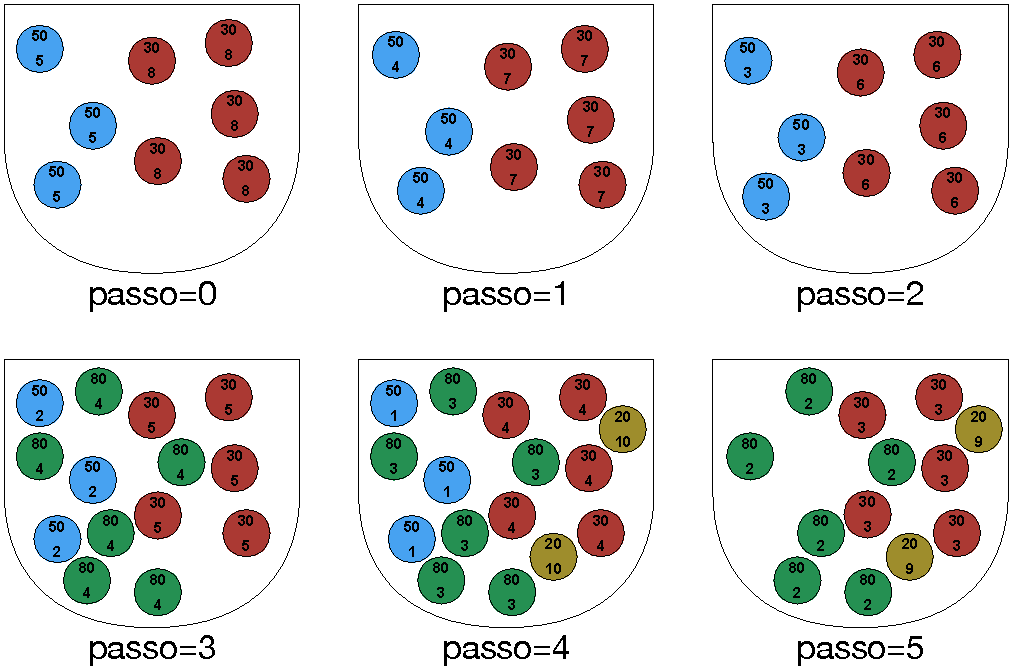
\includegraphics[scale=0.9]{images/BagOfTasks4.pdf}}
	\caption[Exemplo de aplicação \textit{Bag of Tasks}]{Exemplo de aplicação \textit{Bag of Tasks}.}
	\label{ExemploBoT}
\end{figure}

\section{Consolidação de Tarefas}\label{sec:consolidacao_de_tarefas}

A consolidação de tarefas consiste em uma etapa de escalonamento, realizada em nível aplicativo, que realiza o mapeamento das tarefas definidas em uma aplicação sobre um conjunto finito de recursos de processamento. Os critérios de escalonamento para tal consolidação levam em consideração unicamente aqueles atributos empregados para descrever aplicações BoT apresentados na Seção \ref{sec:modelo_de_aplicacao_bot}: data de chegada, duração, número de tarefas, quantidade de processamento requerida e o número de processadores disponíveis.

Assume-se que as seguintes situações possam ser verdadeiras em um determinado instante de execução:

\begin{itemize}
\item O número total de tarefas é maior que o total de processadores disponíveis.
\item A quantidade de processamento requerida pelo conjunto de \textit{jobs} aptos a executar é superior àquela oferecida pelo conjunto de processadores disponíveis.
\end{itemize}

\subsection{Discretização das tarefas}\label{subsec:discretizacao_de_tarefas}

Embora em uma aplicação do tipo BoT inexistam relações de dependência, tampouco precedência entre tarefas, uma tarefa qualquer pode gerar novas tarefas para o bag. Assim, considere duas tarefas $\tau_k^i$ e $\tau_l^j$, definidas em duas quádruplas $q_i$ e $q_j$, de tal forma que $a_i < a_j$, existindo, portanto, um valor $\delta$ tal que $a_i+\delta=a_j$. Isto significa que, pelo menos uma tarefa em $q_i$ pode ter criado $q_j$ ao final da execução de um \textit{job} $w^{\tau^i}_\delta$. Como o modelo de aplicação BoT adotado não distingue as tarefas pertencentes a uma mesma quádrupla, assume-se que todas as tarefas $\tau_l$ de $q_j$ são inseridas no bag após o término do passo $w_{\delta}$ de todas as tarefas $\tau_k$ de $q_i$.

Define-se \emph{passo global} $g$ um instante de tempo discreto na evolução de uma aplicação BoT no modelo descrito em um ambiente com número não limitado de recursos de processamento e sem contenção. Uma aplicação qualquer, descrita por $n$ quádruplas possui $|g| = \max_{i=1}^{k}(a_i+d_i)$ passos globais. Nesta situação, a passagem de $g_i$ para $g_{i+1}$ marca o término da execução de um \textit{job} de cada tarefa presente no bag até $g_i$, inclusive.

Os atributos de um \textit{job} $w_j^i$, criado a partir de uma tarefa $\tau^i_k$ especificada em uma quádrupla $q_i$, são descritos por uma quádrupla contendo $[g_j^i,r_j^i,f_j^i,c_j^i]$, onde $g_j^i$ corresponde ao passo global em que o \textit{job} encontra-se disponível para execução e $c_j^i$ ao custo do \textit{job} definido pela tarefa. Nesta quádrupla, os membros $r_j^i$ e $f_j^i$, respectivamente, representam o número de \textit{jobs} de $\tau_i$ que ainda estão no bag e os que já foram concluídos. Para um dado \textit{job} $w_j^i$, $g_j^i = a_i+f_j^i$, bem como $r_j^i + f_j^i = b_i$ e $c_j^i = c_i$.

Para uma determinada tarefa $\tau^i_k$, são instanciados $d_i$ \textit{jobs} na forma: 

\[\{w_1^i, w_2^i, \dots w_{d_i}^i\} = \{[g_1^i,r_1^i,f_1^i,c_1^i],[g_2^i,r_2^i,f_2^i,c_2^i], [g_3^i,r_3^i,f_3^i,c_3^i] \dots [g_{d_i}^i,r_{d_i}^i,f_{d_i}^i,c_{d_i}^i]\}\]

Para efeito de consolidação das tarefas, assume-se como unidade de manipulação o \textit{job}. Os \textit{jobs} definidos por diferentes tarefas são independentes entre si. Os \textit{jobs} definidos por uma tarefa, no entanto, são executados na ordem expressa pelos respectivos $g_i$.

\subsection{Contingenciamento de execução}\label{subsec:contingenciamento_de_execucao}

Em um ambiente real, a capacidade de processamento é limitada, tanto em termos de recursos, definidos pelo número de processadores ou quantidade de memória, como em termos de capacidade, exemplificada pela velocidade de comunicação. A aplicação em execução, em tais sistemas, é a principal fonte de consumo destes recursos, não sendo, no entanto, a única. A atuação de um sistema de gerenciamento, como o provido pelo mecanismo de escalonamento, também consome a capacidade de processamento oferecida. No modelo BoT apresentado, é considerado apenas o custo computacional de cada tarefa, o que implica em considerar a carga de processamento oferecida pela arquitetura disponível, assumindo, desta forma, ilimitada capacidade de processamento, armazenamento e nulos os custos de comunicação. Assume-se, também, que a influência do mecanismo de escalonamento não introduz sobrecustos à execução.

O número de processadores disponíveis na arquitetura real delimita, no modelo adotado, a capacidade de processamento disponível. Uma arquitetura $M$ dedicada à execução de uma aplicação BoT $A$ é composta por $m$ processadores idênticos, $\{p_1, p_2 \dots p_m\}$, com ilimitada capacidade de memória por processador e custo 0 (zero) para comunicação de tarefas e operações de escalonamento entre eles. Em determinado passo global, a quantidade de processamento máximo disponível nesta máquina é dado por $C = m\times 100\%$.

O número de \textit{jobs} que podem ser executados em um determinado passo global $g$ é limitado pela quantidade de processamento oferecida. Assim, se em um determinado passo global $g$ o somatório dos custos computacionais $c_k^i$ dos \textit{jobs} $w_i$ aptos à execução suplantar a capacidade $C$ de processamento oferecida, haverá contenção na execução. Deve também ser observado que a necessidade de processamento de um \textit{job} não pode ser dividida entre processadores. Como consequência, pode ocorrer fragmentação de uso de processador quando, em um passo global, um novo \textit{job} não pode ser adicionado aos demais por ultrapassar o limite de uso de 100\% de CPU máximo previsto por passo. Assim, a capacidade real $C_g$ explorada em um passo global $g$ é limitada em $C_g \le m\times 100\%$.

\subsection{Normalização do passo global}\label{subsec:normalizacao_do_passo_global}

Como existe contingenciamento na execução dos \textit{jobs}, em função da carga computacional disponível, em um dado passo global $g$ nem todos os \textit{jobs} elegíveis para execução podem ser de fato executados. Assim, cada tarefa terá, no máximo um \textit{job} em execução, havendo a possibilidade de tarefas não terem nenhum \textit{job} executado em um determinado passo global.

Para cada tarefa $\tau^i_k$, apenas um \textit{job} é elegível para execução, sendo este o \textit{job} que possuir o menor $g_j^i$, satisfazendo $g_j^i \le g$. Considerando dois \textit{jobs} $w_j^i$ e $w_k^i$ definidos por uma mesma tarefa $\tau_i$ a relação de ordem temporal definida pelo atributo $g_i$ de cada um deles deve ser preservada.

Considerando dois \textit{jobs} $w_j^i$ e $w_k^h$, definidos pelas tarefas $\tau^i_k$ e $\tau^h_l$, respectivamente, ambas elegíveis para execução, não existe nenhuma ordem pré-definida de execução entre eles.

Em consequência do contingenciamento, em um dado passo $g$ pode existir um conjunto não vazio de \textit{jobs} em que se verifica que $g_i \le g$. Uma parcela limitada das tarefas já iniciadas contendo estes \textit{jobs} é elegível para execução em função da limitação dos recursos de processamento disponíveis. As demais, não elegíveis por não haver recursos de processamento suficientes, terão sua execução retardada.

Deste fato destaca-se a consequência da contingência no modelo de BoT adotado. Conforme previsto na Seção \ref{sec:modelo_de_aplicacao_bot}, o atributo $a_i$ definido por uma quádrupla $q_i$ representa a quantidade de processamento já realizada pela aplicação em uma arquitetura não contingenciada. Portanto, todo atraso na execução de qualquer \textit{job} reflete no atraso, na mesma proporção, da chegada de um novo lote de tarefas (e seus \textit{jobs} correspondentes) da mesma aplicação.

A Figura \ref{fig:normalizatempo} apresenta um exemplo da situação. Supondo duas aplicações $A = \{[0,5,1,c^A_1], [3,d^A_1,2,c^A_1]\}$ e $B = \{[3,d^B_1,3,c^B_1]\}$, cujos atributos não identificados são irrelevantes para compreensão do exemplo. Nesta figura, \textit{jobs} são representados por círculos, sendo envolvidos pelas tarefas que os descrevem. O inteiro informado no interior de cada \textit{job} refere-se ao seu passo de execução. As setas tracejadas identificam a dependência de criação de tarefas anotada entre os \textit{jobs}. A discretização do tempo (passos) também é apresentada.

\begin{figure}[htbp]
	\centerline{
		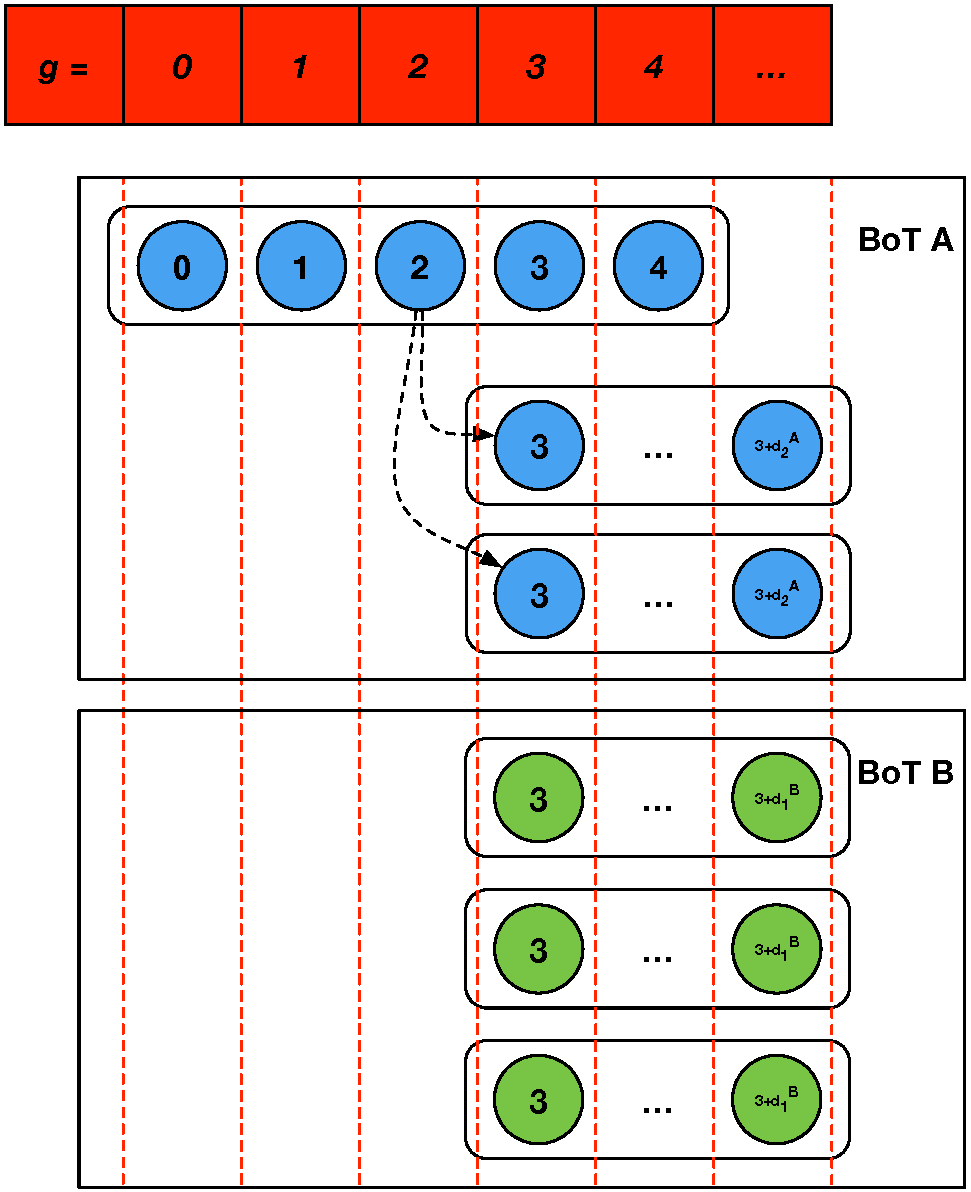
\includegraphics[scale=0.44]{images/NormalizacaoTempo2.pdf}}
	\caption[Dependência na criação de tarefas entre \textit{jobs}.]{Dependência na criação de tarefas entre \textit{jobs}.}
\label{fig:normalizatempo}
\end{figure}

Na Figura \ref{fig:normalizatempo}, o BoT $A$ possui dois grupos de tarefas, o primeiro é recebido no tempo 0 (zero), sendo composto por uma (1) tarefa com comprimento de cinco passos, ou seja, de cinco \textit{jobs}. O segundo grupo é composto por duas tarefas, sendo recebido no tempo 3 em uma arquitetura sem contenção. A interpretação é a de que de todas as tarefas lançadas anteriormente, na mesma aplicação, devem ter tido o direito de executar até 3 passos, ou seja, até 3 de seus \textit{jobs}, de forma que a quantidade de trabalho suficiente para criação deste segundo grupo tenha sido completada.

Nesta mesma figura, o BoT $B$, possui um único grupo de tarefas, composto por três tarefas, que é recebido no tempo 3. A execução destas tarefas não depende de trabalhos realizados em outra aplicação, uma vez que trata-se de um novo BoT. Seus \textit{jobs} não são atrasados, portanto, em decorrência de atrasos de execução de \textit{jobs} descritos em outro BoT, no caso da figura, das tarefas do BoT $A$. \info{Aqui TERMINA o texto que veio da dissertação}

\section{Fontes de Custos em IaaS}\label{sec:fontescustos}
De um modo geral, os custos associados à utilização dos recursos computacionais disponibilizados por nuvens do tipo IaaS são difíceis de ser quantificados, fazendo com que seja necessária a utilização de modelos de decisão orientados a custos. Um dos modelos mais utilizados é o custo total de propriedade -- TCO (\emph{Total Cost of Ownership}) \cite{strebelEconomicDecisionModel2010}.

O custo total de propriedade, inicialmente definido pela empresa Gartner, Inc.\footnote{\url{https://www.gartner.com/en} - empresa criada no final dos anos 1970, com atuação nos ramos de pesquisa, consultoria, eventos e prospecção do mercado de Tecnologia da Informação.}, é reconhecido como o método padrão para a análise financeira de recursos de Tecnologia da Informação (TI) e outros custos empresariais relacionados à TI \cite{mieritzDefiningGartnerTotal2005}. O modelo de TCO inclui aquisição, gerenciamento e suporte de hardware e software, comunicações, despesas do usuário final e os custos com tempo de inatividade, treinamento e outras perdas de produtividade. Para Filiopoulou e seu grupo \cite{filiopoulouIntegratingCostAnalysis2015}, a estimativa do custo total de propriedade, em particular, é um procedimento que fornece os meios para determinar o valor econômico total de um investimento, incluindo as despesas iniciais de capital (CAPEX, \emph{capital expenditure}) e as despesas operacionais (OPEX, \emph{operational expenditure}). No contexto de computação em nuvem, corresponde à estimativa de valores necessários para implementação e operação de uma infraestrutura.

Os benefícios do uso da abordagem de TCO estão na melhoria da comunicação entre cliente e provedor e na análise de todo o ciclo de vida dos artefatos de TI. Além disso, é possível analisar os custos ou componentes de custos individuais de um artefato de TI por meio de um esquema predefinido \cite{walterbuschEvaluatingCloudComputing2013}. Como o objetivo do modelo TCO é fornecer uma visão abstrata e simplificada do ``mundo real'', em vez de incluir todos os custos relevantes na análise, a complexidade da realidade pode ser reduzida trabalhando com base em premissas e incluindo apenas um número limitado de fatores de custo cuidadosamente selecionados.

Métricas para os cálculos de custo e investimento em infraestruturas de nuvens computacionais necessitam de um modelo claro, juntamente com os fatores que influenciam estes custos. A Tabela \ref{tab:tiposfatores} atribui fatores de custo $f$ para cada tipo de custo $t$ identificado. Os tipos de custo $t \in T$ e os fatores de custo $f \in F$ estão sujeitos aos conjuntos $T$ e $F$:
\begin{equation}
  \begin{aligned}
    T = {} & \{dEst,ava,txIaaS,imp,sup,trein,manut,falha,bs\}
  \end{aligned}
\end{equation}
% \myequations{teste}

\begin{equation}
  \begin{aligned}
    F = {} & \{dTempo,sCon,itDec,pComp,cArm,\\ 
          & tEnt,tSda,tInt,nCon,dom,ssl,lic,txServ,\\
          & pPort,cSup,rProb,tPrep,tPart,mInstr,perda\}
  \end{aligned}
\end{equation}

Cada fator influenciador é atribuído a um tipo de custo e, em seguida, os elementos dos conjuntos $T$ e $F$ são agrupados em fórmulas. Cada fórmula é aplicada a um custo específico, possibilitando a obtenção dos valores para cada tipo de custo.

\begin{table}[htb]
  \footnotesize
  \centering
  \caption{Tipos de custo e fatores de custo relacionados}
  \label{tab:tiposfatores}
%   \setlength\tabcolsep{1.6pt} % ajusta a tabela para caber na coluna
  \begin{tabular}{@{}lm{6.9cm}@{}}
    \toprule
    \multicolumn{1}{c}{\textbf{Tipo de custo}} & \multicolumn{1}{c}{\textbf{Fatores de custo}} \\ 
    \bottomrule
    \begin{tabular}[c]{m{7cm}@{}l@{}}Decisão estratégica, seleção de serviços de computação em nuvem e tipos de nuvem (\emph{dEst})\end{tabular} & Despesas de tempo (\emph{dTempo}), serviços de consultoria (\emph{sCon}), informações para tomada de decisão (\emph{itDec}). \\ 
    \addlinespace[0.15cm]
    \begin{tabular}[c]{m{7cm}@{}l@{}}Avaliação e seleção de prestador de serviços (\emph{ava})\end{tabular} & Despesas de tempo (\emph{dTempo}), serviços de consultoria (\emph{sCon}), informações para tomada de decisão (\emph{itDec}).\\ 
    \addlinespace[0.15cm]
    \begin{tabular}[c]{m{7cm}@{}l@{}}Taxa de serviço IaaS (\emph{txIaaS})\end{tabular} & Poder de computação (\emph{pComp}), capacidade de armazenamento (\emph{cArm}), transferência de dados de entrada (\emph{tEnt}), transferência de dados de saída (\emph{tSda}), transferência de dados interna do provedor (\emph{tInt}), número de consultas (\emph{nCon}), domínio (\emph{dom}), certificado SSL (\emph{ssl}), licença (\emph{lic}), taxa de serviço básica (\emph{txServ}). \\
    \addlinespace[0.15cm]
    \begin{tabular}[c]{m{7cm}@{}l@{}}Implementação, configuração, integração e migração (\emph{imp})\end{tabular} & Despesas de tempo (\emph{dTempo}), processo de portabilidade (\emph{pPort}). \\
    \addlinespace[0.15cm]
    \begin{tabular}[c]{m{7cm}@{}l@{}}Suporte (\emph{sup})\end{tabular} & Despesas de tempo (\emph{dTempo}), custos de suporte (\emph{cSup}), resolução de problemas (\emph{rProb}). \\
    \addlinespace[0.15cm]
    \begin{tabular}[c]{m{7cm}@{}l@{}}Treinamento inicial e permanente (\emph{trein})\end{tabular} & Tempo de preparação dos funcionários internos (\emph{tPrep}), tempo de participação dos funcionários internos (\emph{tPart}), material de instruções (\emph{mInstr}), serviços de consultoria externa (\emph{sCon}). \\
    \addlinespace[0.15cm]
    \begin{tabular}[c]{m{7cm}@{}l@{}}Manutenção e modificação (\emph{manut})\end{tabular} & Despesas de tempo (\emph{dTempo}). \\
    \addlinespace[0.15cm]
    \begin{tabular}[c]{m{7cm}@{}l@{}}Falha no sistema (\emph{falha})\end{tabular} & Perda por período (\emph{perda}). \\
    \addlinespace[0.15cm]
    \begin{tabular}[c]{m{7cm}@{}l@{}}\emph{Backsourcing} ou descarte (\emph{bs})\end{tabular} & Despesas de tempo (\emph{dTempo}), processo de portabilidade (\emph{pPort}). \\  
    \bottomrule
  \end{tabular}
  \caption*{Fonte: Adaptado de \cite{walterbuschEvaluatingCloudComputing2013}.}
\end{table}

\section{Fatores de Custo}
\label{sec:fatorescustos}

Os custos relacionados à decisão estratégica, seleção de serviços de computação em nuvem e tipos de nuvem (\emph{dEst}), juntamente com os custos de avaliação e seleção de prestadores de serviço (\emph{ava}) são influenciados pelas despesas de tempo (\emph{dTempo}) necessário para a tomada de decisão, as despesas com informações nas quais a decisão pode ser baseada (\emph{itDec}), como, por exemplo literatura científica ou análises de mercado, bem como custos de serviços de consultoria externa (\emph{sCon}). O custo total com as despesas de tempo resultam do tempo total gasto por todos os funcionários $\left(C^{dEst}_{dTempo} = \sum p^{dEst}_{dTempo,m} * a^{dEst}_{dTempo,m}\right)$, ou seja, é determinado pelo valor da hora de trabalho de cada empregado $\left(p^{dEst}_{dTempo,m}\right)$, multiplicado pelo tempo gasto $\left(a^{dEst}_{dTempo,m}\right)$, e somando os valores de todos os empregados $\left(m\right)$ envolvidos. Custos com tomadas de decisão ocorrem em períodos $i < 1$ e, além disso, o custo total com a aquisição de informações (\emph{itDec}) pode ser descrito como o somatório do total de preços (\emph{p}) de todos os materiais adquiridos $\left(C^{dEst}_{itDec} = \sum p^{dEst}_{a}\right)$. Por fim, os custos com serviços de consultoria $\left(C^{dEst}_{sCon}\right)$ são adicionados ao total e todos os gastos correspondentes aos fatores que influenciam o tipo de custo \emph{dEst}, sumarizados pela fórmula $\left(C^{dEst} = C^{dEst}_{dTempo} + C^{dEst}_{sCon} + C^{dEst}_{itDec}\right)$. Para o processo de avaliação e seleção de prestadores de serviços (\emph{ava}), os custos dependem da quantidade de tempo que os empregados dedicam a este processo (\emph{dTempo}) e os custos de eventuais consultorias externas (\emph{sCon}). Os cálculos para $\left(C^{ava}_{dTempo}\right)$ e $\left(C^{ava}_{sCon}\right)$ são análogos a $\left(C^{dEst}_{dTempo}\right)$ e $\left(C^{dEst}_{sCon}\right)$.

Para implementações de nuvem do tipo Infraestrutura como Serviço (IaaS), o tipo de custo que relaciona as taxas sobre os serviços (\emph{txIaaS}) é composto por elementos como o custo com poder de computação (\emph{pComp}), que pode ser calculado multiplicando o número de unidades de processamentos utilizadas $\left(a^{txIaaS}_{pComp,i}\right)$ por período \emph{i}, pelo custo de uma unidade de processamento $\left(p^{txIaaS}_{pComp,i}\right)$. O preço varia de acordo com as características específicas do sistema, como, memória RAM, número de unidades de computação, capacidade de armazenamento, sistema operacional $\left(C^{txIaaS}_{pComp,i} = a^{txIaaS}_{pComp,i} * p^{txIaaS}_{pComp,i}\right)$ e o custo total deste fator \emph{pComp} resulta do somatório de preços durante todos períodos \emph{n} $\left(C^{txIaaS}_{pComp,i} = \sum\limits^{n}_{i=1} C^{txIaaS}_{pComp,i}\right)$. Com a generalização do cálculo $\left(C^{t}_{f,i} = \sum\limits^{n}_{i=1}a^{t}_{f,i} * p^{t}_{f,i}\right)$, que sumariza os custos unitários em função da quantidade consumida em um período de uso \emph{i}, pode-se aplicar o mesmo raciocínio para os valores de capacidade de armazenamento (\emph{cArm}), transferência de dados de entrada (\emph{tEnt}), transferência de dados de saída (\emph{tSda}) e a transferência de dados interna para outros serviços do mesmo provedor (\emph{tInnt}) e o custo com o número de consultas (\emph{nCon}). Os custos com manutenção de domínio para acesso Web (\emph{dom}), certificados SSL (\emph{ssl}), licenciamento de software (\emph{lic}) e taxas básicas de serviços (\emph{txServ}) podem ser determinados pela multiplicação do número de períodos utilizados \emph{n} pelo respectivo preço $p^{t}_{f}$ do fator de custo \emph{f} do respectivo tipo de custo \emph{t} $\left(C^{t}_{f} = n * p^{t}_{f}\right)$.

As despesas com o tempo (\emph{dTempo}) necessário para cumprir as tarefas de implementação, configuração, integração e migração de serviços e dados influenciam o custo total tipo de custo (\emph{imp}). Um fator de custo importante neste tipo de custo é o processo de portabilidade (\emph{pPort}) dos dados do cliente para provedor de serviços. Conforme mencionado, os provedores cobram de seus clientes pela transferência de dados de entrada. Os custos da transferência inicial de dados para a nuvem para fins de migração do sistema pertencem a este tipo de custo. Eles são calculados multiplicando o volume de dados por unidade (ou seja, gigabyte) pelo preço de uma unidade. Alguns provedores oferecem serviços de envio de disco rígido para inserir os dados do cliente. No entanto, essa abordagem não se concentra no volume de dados, mas sim no número de discos rígidos e no tempo de carregamento de dados. O fator de custo de \emph{pPort} não depende de mudanças temporais de preço porque se presume que o processo de portabilidade de dados pode ser concluído dentro de um período \emph{t}: $\left(C^{imp}_{pPort} = a^{imp}_{pPort} * p^{imp}_{pPort}\right)$. As despesas de tempo $C^{imp}_{dTempo}$ podem ser determinadas da mesma maneira que $C^{dEst}_{dTempo}$: $\left(C^{imp}_{dTempo} = \sum p^{imp}_{dTempo,m} * a^{imp}_{dTempo,m}\right)$.

O tipo de custo Suporte (\emph{sup}) depende do custo dos serviços de atendimento via telefone, e-mail, sistema de chamados ou \emph{chat} durante todo ciclo de vida da infraestrutura de nuvem. Portanto, este tipo de custo depende do gasto de tempo (\emph{dTempo}) necessário para interação com a equipe de suporte, bem como dos custos ocorridos. Alguns provedores de serviços cobram seus usuários com base no tempo necessário para a resolução de problemas e suporte. Os custos totais com suporte podem ser determinados pela multiplicação do preços de uma unidade pelo número total de unidades necessárias $\left(C^{sup}_{cSup} = p^{sup}_{cSup} * a^{sup}_{cSup}\right)$. Já os custos com resolução de problemas dependem do número de unidades consumidas e o preço por unidade $\left(C^{sup}_{rProb} = p^{sup}_{rProb} * a^{sup}_{rProb }\right)$.

Os custos totais do tipo de custo "treinamento inicial e permanente" (\emph{trein}) podem ser subdivididos em treinamento interno, no qual os próprios colaborados atuam como treinadores, e treinamento externo, no qual são necessários treinadores externos à empresa. Os custos de um treinamento interno dependem da quantidade de tempo de preparação investido por um ou mais empregados (\emph{tPrep}), o tempo de participação dos funcionários internos (\emph{tPart}) e os custos com material para os treinamentos (\emph{mInstr}):

\begin{eqnarray*}
C^{trein}_{int} &=& \sum C^{trein}_{tPrep,m} + \sum C^{trein}_{tPart,m} + C^{trein}_{mInstr,m} \\
                &=& \sum\left(p^{trein}_{tPrep,m} * a^{trein}_{tPrep,m}\right) \\
                &+& \sum\left(p^{trein}_{tPart,m} * a^{trein}_{tPart,m}\right) + C^{trein}_{mInstr}
\end{eqnarray*}

O total dos custos de um treinamento externo pode se calculado pela adição dos custos com serviços de consultoria que organizam o treinamento (\emph{sCon}), a quantidade de tempo que os empregados investem na participação do treinamento (\emph{tPart}) e os custos com materiais de treinamento (\emph{mInstr}):

\begin{eqnarray*}
C^{trein}_{ext} &=& \sum C^{trein}_{sCon} + \sum C^{trein}_{tPart} + C^{trein}_{mInstr,m} \\
                &=& \sum\left(p^{trein}_{sCon} * a^{trein}_{sCon}\right) \\
                &+& \sum\left(p^{trein}_{tPart,m} * a^{trein}_{tPart,m}\right) + C^{trein}_{mInstr}
\end{eqnarray*}

Custos com manutenção e modificação (\emph{manut}) dependem das despesas com tempo gasto (\emph{dTempo}) em manutenções gerais e em modificações feitas para implementação de serviços $\left(C^{manut}_{dTempo}\right)$. O cálculo das despesas de tempo para uma respectiva tarefa de manutenção é baseada na fórmula do tipo de custo \emph{dEst}: $\left(c^{manut}_{dTempo} = \sum p^{dEst}_{dTempo,m} * a^{dEst}_{dTempo,m}\right)$.

Custos totais de uma falha de sistema precisam ser declarados para cada empresa individualmente. Os possíveis fatores de custo são, por exemplo, perda de tempo de trabalho produtivo, penalidades contratuais por atrasos ou danos à reputação da empresa, que são difíceis de mensurar. Assim, apenas destaca-se uma fórmula geral que representa a perda por período \emph{i}:
\begin{eqnarray*}
C^{falha}_{perda} = \sum\limits^{n}_{i=1} a^{falha}_{perda,i} * p^{falha}_{perda,i}
\end{eqnarray*}

O processo de descarte, ou \emph{backsourcing}, de um sistema envolve despesas de tempo (\emph{dTempo}) e processo de portabilidade (\emph{pPort}). No entanto, os custos com a portabilidade dos dados entre nuvens, ou para um sistema diferente, fazem parte do TCO de um novo serviço e não do TCO do sistema no qual os dados estão sendo retirados. Os custos podem ser determinados da mesma maneira que os custos do processo de portabilidade dos dados para a nuvem $\left(C^{bs}_{pPort} = a^{bs}_{pPort} * p^{bs}_{pPort}\right)$ e também dependem do gasto de tempo necessário para a decisão estratégica necessária:
\begin{eqnarray*}
C^{bs}_{dTempo} = \sum p^{bs}_{dTempo,m} * a^{bs}_{dTempo,m}
\end{eqnarray*}

\section{Custo Global}
\label{sec:custoglobal}
Em um ambiente de nuvem pública do tipo IaaS, o custo total de propriedade de um serviço de computação em nuvem é igual à soma de todos os tipos de custos envolvidos e pode ser definido como:

\begin{equation}
  \centering
  \begin{aligned}
    TCO_{Nuvem} = \sum C^t ~\textsf{onde}~ t \in T
  \end{aligned}
  \label{eq:tco}
\end{equation}

O valor total de um tipo de custo $t$ é igual à soma de todos os fatores de custo $f$ envolvidos, conforme segue: $C^t = \sum C^t_f ~\textsf{onde}~ t \in T, f \in F$. 

Neste modelo de TCO é considerado o período total de tempo no qual os serviços de nuvem foram ou serão utilizados. Este período é subdividido em vários períodos menores $i$, com duração de um mês, geralmente, predefinido pelo provedor de serviços. Assim, o período total é composto por $n$ períodos menores, de acordo com $C^t_f = \sum^n_i C^t_{f,i} ~\textsf{onde}~ i = \{1, \dots, n\}, t \in T, f \in F$. As variáveis $a^t_{f,i}$ e $p^t_{f,i}$ são utilizadas, respectivamente, para representar a quantidade consumida ou necessária no período $i$ e caracterizar os custos ou preços unitários na fórmula $C^t_{f,i} = a^t_{f,i} ~\textsf{*}~ p^t_{f,i}$.

Ao contrário de serviços entregues por meio de nuvens públicas, nas estruturas de nuvens privadas os usuários e provedores fazem parte da mesma organização ou os serviços são prestados, de modo exclusivo, por terceiros. No primeiro cenário, os custos envolvidos incluem, por exemplo, licenciamento de softwares implementados bem como a infraestrutura de TI que deve ser fornecida pela organização. Já no caso de entrega de serviços por provedor exclusivo, o fornecimento é semelhante a uma nuvem pública IaaS, no modo em que o usuário obtém os recursos de um provedor. Apesar disso, o provedor não gerencia dados em uma estrutura pública, mas, sim, em uma nuvem privada exclusiva. 

Finalmente, em soluções de nuvens híbridas, que agregam as características de nuvens públicas e privadas, as despesas totais são iguais aos custos totais, ou pelo menos proporcionais, envolvidos em cada solução individual. Além disso, despesas com o processo de agregação de soluções (públicas e privadas) devem ser consideradas na composição dos custos e investimentos.

\section{Aspectos de Custo em Ambientes HPC}\label{sec:custoshpc}

Aplicações para Processamento de Alto Desempenho possuem diferentes características que podem determinar sua adequação a um ambiente de nuvem. Questionamentos a respeito de por que e quem deve escolher uma nuvem para execução de aplicações HPC, quais destas aplicações e como a nuvem pode ser usada para HPC devem balizar os estudos de viabilidade de migração para ambientes remotos distribuídos. 

Ambientes HPC são orientados a desempenho, ao passo que nuvens computacionais são orientadas pela relação custo (monetário) \emph{vs.} utilização de recursos. Além disso, nuvens foram, originalmente, projetadas para a execução de aplicações comerciais e de serviços para a internet. O uso de conexões de rede não apropriadas para alto desempenho, a sobrecarga das técnicas de virtualização e as limitações dos sistemas de armazenamento podem ser considerados barreiras para a adoção de nuvens para aplicações HPC. Cabe, então, identificar \cite{guptaEvaluatingImprovingPerformance2016d}:

\begin{itemize}[noitemsep]
    \item \emph{Quem} é o usuário candidato para um ambiente de nuvem;
    \item \emph{Qual} é o tipo de aplicação que pode se beneficiar de uma execução em ambiente de nuvem;
    \item \emph{Por que} o usuário terá benefícios na execução de sua aplicação em ambiente de nuvem; e,
    \item \emph{Como} este benefício pode ser atingido.
\end{itemize}

Com base nestes pontos, as tabelas \ref{tab:questoes1} e \ref{tab:questoes2} apresentam alguns posicionamentos com relação aos questionamentos originados a partir de duas diferentes abordagens que visam auxiliar nas decisões de migração para ambientes de nuvem computacional: 
\begin{enumerate*}[label=\textit{\alph*}),itemjoin={{; }},itemjoin*={{; e }}]
  \item considera-se os aspectos da execução em modelos de desempenho, custo e negócios
  \item são exploradas técnicas para preencher as lacunas entre nuvens e aplicações HPC
\end{enumerate*}. Estas abordagens têm por objetivo identificar as diferenças de demandas por HPC, por parte dos usuários, e quais alternativas eles dispõem para implantar suas aplicações. As alternativas que buscam preencher a lacuna entre aplicações HPC e nuvens podem ser classificadas em duas categorias \cite{guptaEvaluatingImprovingPerformance2016d}: primeiro, aquelas que objetivam tornar as nuvens cientes das aplicações HPC e, segundo, aquelas que buscam tornar as aplicações HPC cientes das infraestruturas de nuvem nas quais serão executadas.

A Tabela \ref{tab:questoes1} traz respostas para a o cenário no qual é pretendido tornar as nuvens cientes das aplicações HPC que serão executadas. Para isso, são exploradas técnicas de virtualização leve (por exemplo, contêineres) e determina-se quão próximo do desempenho de máquina física é possível chegar com as aplicações HPC. São exemplos, \textit{hypervisors} otimizados para HPC e nuvens otimizadas para computação de alto desempenho como Amazon HPC.

\begin{table}[htb]
  \footnotesize
  \centering
  \caption{Questões sobre nuvens cientes de aplicações HPC}
  \label{tab:questoes1}
%   \setlength\tabcolsep{1.6pt} % ajusta a tabela para caber na coluna
  \begin{tabular}{@{}lm{11.2cm}@{}}
    \toprule
    \multicolumn{1}{c}{\textbf{Questionamento}} & \multicolumn{1}{c}{\textbf{Resposta}} \\ 
    \bottomrule
    \begin{tabular}[c]{@{}l@{}}Quem\end{tabular} & Pequenas e médias organizações ou empresas em crescimento. \\ 
    \addlinespace[0.15cm]
    \begin{tabular}[c]{@{}l@{}}Qual\end{tabular} & Aplicações com padrões de comunicação menos intensos e menos sensíveis a interferências. \\ 
    \addlinespace[0.15cm]
    \begin{tabular}[c]{@{}l@{}}Por que\end{tabular} & Pequenas e médias organizações que são sensíveis aos argumentos de CAPEX/OPEX. \\
    \addlinespace[0.15cm]
    \begin{tabular}[c]{@{}l@{}}Como\end{tabular} & Tornar as nuvens cientes das aplicações HPC, por exemplo, com uso de virtualização leve e afinidade de CPU. \\ 
    \bottomrule
  \end{tabular}
  \caption*{Fonte: Adaptado de \cite{guptaEvaluatingImprovingPerformance2016d}.}
\end{table}

Já na Tabela \ref{tab:questoes2}, as respostas tratam de pontos que devem ser considerados quando se busca por ambientes de execução capazes de trabalhar com aplicações HPC cientes de nuvens computacionais. Esta alternativa, embora ainda pouco explorada, permite ajustes nos tempos de execução das aplicações HPC em nuvens para obtenção de um melhor desempenho com uso de tecnologias como balanceadores de carga com reconhecimento de nuvem para aplicações HPC e a implantação de topologias com reconhecimento de aplicações científicas na nuvem.

\begin{table}[htb]
  \footnotesize
  \centering
  \caption{Questões sobre aplicações HPC cientes de nuvem}
  \label{tab:questoes2}
%   \setlength\tabcolsep{1.6pt} % ajusta a tabela para caber na coluna
  \begin{tabular}{@{}lm{11.2cm}@{}}
    \toprule
    \multicolumn{1}{c}{\textbf{Questionamento}} & \multicolumn{1}{c}{\textbf{Resposta}} \\ 
    \bottomrule
    \begin{tabular}[c]{@{}l@{}}Quem\end{tabular} & Usuários com aplicações que tem melhor relação custo/desempenho em nuvens \textit{vs.} outras plataformas. \\ 
    \addlinespace[0.15cm]
    \begin{tabular}[c]{@{}l@{}}Qual\end{tabular} & Aplicações com necessidades de desempenho que podem ser atendidas em média escala (em termos de número de \textit{cores}). \\ 
    \addlinespace[0.15cm]
    \begin{tabular}[c]{@{}l@{}}Por que\end{tabular} & Nuvens permitem que vários usuários acessem estruturas compartilhadas, garantindo um melhor uso dos recursos. \\
    \addlinespace[0.15cm]
    \begin{tabular}[c]{@{}l@{}}Como\end{tabular} & Abordagem híbrida supercomputador-nuvem com escalonamento ciente de aplicação e \textit{cloud bursting}. \\ 
    \bottomrule
  \end{tabular}
  \caption*{Fonte: Adaptado de \cite{guptaEvaluatingImprovingPerformance2016d}.}
\end{table}

O uso de nuvens para execução de aplicações HPC pode ser visto como um bom complemento para estruturas locais de supercomputadores e \textit{clusters}, não podendo, ainda, substituí-las totalmente. Abordagens de utilização de nuvens híbridas, nas quais ocorre uma integração entre infraestruturas de nuvens públicas e privadas, permitem a ocorrência de \emph{cloud bursting} \cite{mansouri_automated_2020}. Isto faz com que aplicativos utilizem toda a capacidade dos recursos computacionais de uma nuvem privada e, em reação a este aumento, migrem suas tarefas em ambientes de nuvem pública, à medida que os recursos locais se tornem escassos.

Aplicações científicas tem necessidades significativamente diferentes das aplicações comerciais típicas, executando suas tarefas de maneira fortemente acoplada e em escalas bem maiores de recursos computacionais. Tal comportamento leva a requisitos de largura de banda e latência mais exigentes do que a maioria dos usuários de nuvem. Aplicações científicas também requerem acesso a grandes quantidades de dados e isso pode levar a um grande custo de inicialização e armazenamento \cite{magellan_report_2011}.

Cargas de trabalho científicas podem ser classificadas em três categorias abrangentes de acordo com seus requisitos: fortemente acopladas em grande escala, médio alcance e alto rendimento. A Tabela \ref{tab-reccloud} apresenta características que favorecem o entendimento da viabilidade de execução de aplicações HPC em nuvens. Também classifica, em alto nível, cargas de trabalho executadas pela comunidade científica.

\begin{table}[htb]
  \footnotesize
  \centering
  \caption{Recomendação de uso de nuvens em função do tipo de aplicação HPC}
  \label{tab-reccloud}
%   \setlength\tabcolsep{1.6pt} % ajusta a tabela para caber na coluna
  \begin{tabular}{@{}lm{11.1cm}@{}}
    \toprule
    \multicolumn{1}{c}{\textbf{Tipo de Aplicação}} & \multicolumn{1}{c}{\textbf{Recomendação}} \\ 
    \bottomrule
    \begin{tabular}[c]{@{}l@{}}Fortemente acoplada\\ em grande escala\end{tabular} & Tipicamente, aplicações MPI, que utilizam milhares de \textit{cores} e exigem uma rede de comunicação de alto desempenho. Neste caso, qualquer gargalo de virtualização  ou problemas de alta latência na rede terão impacto negativo no desempenho das aplicações. Logo, é recomendável a execução em ambientes tradicionais de supercomputação ou em nuvens privadas com servidores \textit{bare metal} e redes de alta velocidade. \\ 
    \addlinespace[0.15cm]
    \begin{tabular}[c]{@{}l@{}}Médio alcance\end{tabular} & Estas aplicações utilizam um número variado de \textit{cores} (dezenas ou centenas) e têm requisitos de desempenho mais baixos do que as aplicações de grande escala fortemente acopladas. Consequentemente, são mais tolerantes à virtualização e redes tradicionais. É recomendado que estas aplicações explorem os benefícios do acesso rápido a recursos para a nuvem, especialmente a virtualização leve (contêineres). \\ 
    \addlinespace[0.15cm]
    \begin{tabular}[c]{@{}l@{}}Alto rendimento\end{tabular} & Aplicações  compostas por tarefas independentes que exigem pouca ou nenhuma comunicação. Tais aplicações podem se beneficiar de um grande número de recursos disponíveis e são tolerantes à heterogeneidade. Recomenda-se o uso de nuvens para estas aplicações, especialmente explorando mecanismos de elasticidade. Outros benefícios também podem ser alcançados por meio de ambientes de nuvem híbrida HPC, distribuindo tarefas em \textit{clusters} locais e nuvens públicas. \\ 
    \bottomrule
  \end{tabular}
  \caption*{Fonte: Adaptado de \cite{magellan_report_2011}.}
\end{table}

A partir da classificação das cargas de trabalho científicas, caracterizadas anteriormente (Tabela \ref{tab-reccloud}), é possível identificar alguns exemplos de cada um dos tipos de aplicação, conforme descrito na Tabela \ref{tab-exemplos}.

\begin{table}[htb]
  \footnotesize
  \centering
  \caption{Exemplos de aplicações HPC}
  \label{tab-exemplos}
%   \setlength\tabcolsep{1.6pt} % ajusta a tabela para caber na coluna
  \begin{tabular}{@{}lm{11.1cm}@{}}
    \toprule
    \multicolumn{1}{c}{\textbf{Tipo de Aplicação}} & \multicolumn{1}{c}{\textbf{Exemplos}} \\ 
    \bottomrule
    \begin{tabular}[c]{@{}l@{}}Fortemente acoplada\\ em grande escala\end{tabular} & Aplicações MPI; aplicações de geração de modelos climáticos, sísmicos. \\ 
    \addlinespace[0.15cm]
    \begin{tabular}[c]{@{}l@{}}Médio alcance\end{tabular} & Aplicações de simulação orientada a eventos; aplicações escalonadas no tempo, cujos trabalhos são menos sensíveis a prazos. \\ 
    \addlinespace[0.15cm]
    \begin{tabular}[c]{@{}l@{}}Alto rendimento\end{tabular} & Aplicações BoT; aplicações MapReduce; simulações Monte Carlo. \\ 
    \bottomrule
  \end{tabular}
\end{table}

Em seu estudo, o grupo de Parashar \cite{parashar_cloud_2013} apresentou uma divisão dos ambientes de nuvem para HPC em três categorias:
\begin{enumerate*}[label=\textit{\alph*}),itemjoin={{; }},itemjoin*={{; e }}]
  \item \textbf{{\itshape HPC in the Cloud}}, que se concentra em mover aplicações HPC para ambientes de nuvem
  \item \textbf{{\itshape HPC Plus Cloud}}, na qual usuários fazem uso de nuvens para complementar seus recursos de HPC, em situações de picos de demanda (\textit{cloud bursting})
  \item \textbf{{\itshape HPC as a Service}}, que expõe os recursos HPC por meio de serviços de nuvem
\end{enumerate*}. Estas categorias estão relacionadas a como os recursos são alocados e abstraídos para simplificar o uso da nuvem.

A execução de aplicações HPC em nuvem ainda possui vários problemas em aberto. Para exemplificar, a abstração da infraestrutura de nuvem limita o ajuste das aplicações.  Além disso, a maioria das conexões de rede dos provedores de nuvem não é rápida o suficiente para aplicações fortemente acopladas em grande escala, com alta comunicação entre processadores. 

O modelo de negócio para uma nuvem HPC também é um campo a ser bem explorado. Em nuvens públicas, provedores de serviços lançam várias cargas de trabalho sobre os mesmos recursos físicos a fim de explorar economia de escala, que nem sempre é apropriada para HPC. Além disso, mesmo que pequenas empresas se beneficiem do rápido acesso a recursos de nuvens públicas, isso nem sempre é verdadeiro para grandes usuários de HPC \cite{netto_hpc_2018}. 

Por outro lado, em ambientes de nuvens privadas, usuários de HPC podem ter acesso direto ao gerenciamento dos componentes e o compartilhamento de recursos é reduzido por consequência de o modelo de múltiplos inquilinos ficar limitado a um grupo específico de usuários.

Questões referentes à troca de CAPEX por OPEX tem destaque no processo de decisão de migração de aplicações para ambientes de nuvem. CAPEX está relacionado com os investimentos feitos na aquisição de equipamentos, softwares e inicialização dos mesmos dentro do provedor de serviço. Já o OPEX diz respeito aos investimentos feitos com alocação de serviços, como por exemplo, manutenção de equipamentos e contratação de serviços de nuvem. 

Aplicações que fazem uso variável dos recursos computacionais determinam uma menor utilização global dos equipamentos. Juntamente com os pontos referentes a CAPEX e OPEX, esta utilização variável de recursos serve de argumentos para provedores e usuários finais de nuvem. Os usuários podem se beneficiar caso suas execuções se caracterizem como aplicações de uso variável \cite{guptaEvaluatingImprovingPerformance2016d}. Por outro lado, provedores de nuvem podem tirar benefícios de uma utilização agregada de recursos de todos os seus inquilinos. Para isso, é fundamental que a agregação possa sustentar um modelo de precificação lucrativo frente aos grandes investimentos iniciais necessários para oferecer recursos de computação e armazenamento por meio de uma interface em nuvem pública. No caso de uma nuvem privada, o lucro está em oferecer mais produtividade para os usuários, atendendo de modo satisfatório às demandas da instituição.

\section{Discussão}\label{sec:discussao}

Aplicações HPC necessitam de muitos recursos computacionais e fornecê-los de maneira otimizada requer ajustes em vários aspectos \cite{GantikowReichKnahletal.2015}. Em termos de desempenho, o uso de virtualização já está bem mais aprimorado, devido ao suporte à virtualização no nível de sistema operacional, fornecendo desempenho próximo às infraestruturas de \textit{bare-metal}.

Do ponto de vista do fluxo de trabalho, a transição de uma infraestrutura de hardware dedicado para serviços oferecidos em nuvem implica em uma modificação de processos. Isto é válido para qualquer tipo de aplicação, inclusive para as aplicações HPC. Esta mudança de processo é especialmente complicada devido ao armazenamento e à transferência de grandes quantidades de dados. Este aspecto pode ser simplificado com a hospedagem dos dados diretamente no provedor de serviços.

Os ambientes de nuvem e as estruturas clássicas para HPC têm maneiras distintas de gerenciar recursos de computação. Para extrair o melhor desempenho de um ambiente em nuvem, os esforços concentraram-se em aumentar o isolamento entre máquinas virtuais e reduzir a sobrecarga imposta pelas técnicas de virtualização. As estruturas HPC, por sua vez, visam extrair o máximo de desempenho possível da infraestrutura \cite{netto_hpc_2018}. 

As solicitações de usuários para acessar exclusivamente partes de um \textit{cluster} HPC são enfileiradas sempre que os recursos estiverem sobrecarregados. Em ambientes de nuvem isso não ocorre devido à disponibilidade ``ilimitada'' de recursos, também chamada de elasticidade. Além do mais, hardware para HPC, especificamente interfaces de rede, são consideravelmente mais caras do que exemplares utilizados para criação de nuvens tradicionais, com hardware de \textit{commodity}\footnote{Em um contexto de Tecnologia da Informação, é um dispositivo ou componente de dispositivo que é relativamente barato, amplamente disponível e, em alguns casos, intercambiável com outro hardware do mesmo tipo.}. Sendo assim, alocar usuários em hardwares específicos para HPC, configura um desperdício para o provedor de serviços, caso ele não atenda exclusivamente usuários com demandas HPC.

O desafio em gerenciar recursos HPC em nuvens está em desenvolver um modelo de negócio sustentável, com economia de escala e que ofereça processamento de alto desempenho aos usuários. Para avançar nesta área, esforços de pesquisa devem ser concentrados para que os provedores possam oferecer sistemas de filas e modelos de preços que levem em conta o tempo que os usuários estão dispostos a esperar para ter acesso aos recursos. Alguns modelos flexíveis de aluguel de recursos HPC em nuvens, como apresentado em \cite{zhaoDesigningFlexibleResource2012e}, são baseados em estratégias de planejamento que consideram instâncias sob demanda e \textit{spot}, motivados pelos interesses das duas partes, usuário e provedor, envolvidas no processo de alocar recursos.

\chapter{Trabalhos Relacionados e Estado da Arte}\label{chap:trabEst}

Neste capítulo é apresentada a Revisão Sistemática da Literatura (RSL), juntamente com os trabalhos relacionados ao tema deste estudo. A Seção \ref{sec:sintese} sintetiza os resultados da RSL, respondendo as questões de pesquisa a partir dos trabalhos restantes do processo de revisão. Desta síntese, aponta-se oportunidades de pesquisa na Seção \ref{sec:oportunidades} A Seção \ref{sec:trabrel} encerra o capítulo apresentando uma discussão sobre os trabalhos relacionados selecionados a partir da RSL realizada.

\section{Revisão Sistemática}\label{sec:revisao}

No processo de pesquisa e seleção dos trabalhos relacionados ao tema deste estudo, foi realizada uma Revisão Sistemática da Literatura, desenvolvendo seus três grandes estágios: planejamento, condução e relatório da revisão \cite{xiaoGuidanceConductingSystematic2017a}. Na fase de planejamento, é identificada a necessidade de uma revisão, com a especificação de questões de pesquisa e desenvolvimento de um protocolo de revisão. Na condução da revisão, são identificados e selecionados os estudos primários, extraídos os dados, analisados e sintetizados. Por fim, no relatório da revisão sistemática, são divulgadas as descobertas e discutidos os trabalhos restantes da pesquisa.

\subsection{Planejamento da RSL}\label{sec:planejamentoRSL}

Para o desenvolvimento da RSL no tema proposto, durante o estágio de planejamento, foram definidas algumas Questões de Pesquisa (QPs) com o objetivo de nortear e fundamentar o estudo. As Questões de Pesquisa são:

\textbf{QP 1: Qual o impacto econômico nas decisões de implantação de aplicações de alto desempenho em nuvens computacionais?}

Esta QP busca identificar como instituições (acadêmicas ou comerciais) podem se beneficiar do uso de nuvens computacionais para execução de aplicações que demandem alto poder de processamento. Esta questão considera os custos financeiros envolvidos.

\textbf{QP 2: Como os usuários podem identificar qual a melhor configuração de nuvem, seja pública ou privada, para executar suas aplicações?}

Nesta questão, o objetivo é prover subsídios para que os usuários de nuvem possam determinar qual opção de configuração, oferecida pelos provedores de serviço, mais se adapta às necessidades de suas demandas de processamento. Neste aspecto deve ser levado em conta que existe perda financeira à medida que houver super ou subdimensionamento de recursos.

\textbf{QP 3: Quais modelos de custo financeiro são empregados na execução de aplicações de alto desempenho em nuvens?}

Com esta questão, busca-se identificar possíveis modelos de custo utilizados por instituições para definir as demandas de  infraestruturas de nuvem para execuções de aplicações com demanda de processamento de alto desempenho.

\textbf{QP 4: Como identificar eventuais perdas financeiras em função de imprecisão no dimensionamento de infraestruturas de nuvens para aplicações com demandas de HPC?}

O objetivo desta questão é identificar se haverá perda financeira em função do dimensionamento inadequado da infraestrutura para a demanda do usuário. Neste caso, pode ocorrer superdimensionamento, sendo dispendidos mais recursos na infraestrutura que o necessário para atender à demanda, ou subdimensionamento, quando a execução da aplicação pode atrasar devido à insuficiência de recursos computacionais para atender à demanda. No primeiro caso, a perda está relacionada ao passivo em recursos instalados, e as consequentes despesas em manutenção. No segundo, a perda está relacionada ao baixo índice de produção e a consequente perda de lucros.

De posse destas Questões de Pesquisa, foi realizada uma busca exploratória à procura de trabalhos que abordassem os principais temas contidos nas perguntas. Com isso foi possível identificar como a comunidade científica faz referência aos temas e também extrair palavras-chave utilizadas para composição da \emph{string} de busca utilizada na presente RSL, conforme documentado na sequência (Seção \ref{sec:conducaoRSL}).

\subsection{Condução da RSL}\label{sec:conducaoRSL}

Para a condução desta RSL foram acessadas diversas bases de indexação de trabalhos, amplamente utilizadas por pesquisadores. Ao todo foram selecionadas cinco bases:
\begin{enumerate*}[label=\textit{\roman*}),itemjoin={{; }},itemjoin*={{; e }}]
  \item ACM Digital Library
  \item IEEE Digital Library
  \item Science@Direct
  \item Scopus
  \item Web of Science
\end{enumerate*}. Tais bases foram escolhidas devido a sua importância e por serem repositórios digitais que oferecem acesso eletrônico à maioria dos periódicos e artigos de conferências publicados na área da Ciência da Computação. \cite{okoliGuideConductingSystematic2010}.

Em seguida, um conjunto de termos de pesquisa foi identificado para compor a \emph{string} de busca com a qual será possível extrair da literatura trabalhos relacionados com o tema abordado. Os termos selecionados visam identificar, na literatura, trabalhos envolvendo ambientes de nuvens (\emph{(cloud OR ``cloud computing'')}) e computação de alto desempenho (\emph{(hpc OR ``high performance computing'')}). A esta \emph{string} foram associados termos referentes a possíveis modelos de custo e preços praticados em situações que contemplem a execução de aplicações de HPC em ambientes de nuvem, analisando sua viabilidade financeira (\emph{(``cost model'' OR ``cost efficiency'' OR ``cost analysis'' OR ``economic analysis'' OR ``monetary cost'' OR ``billing model'' OR ``price efficiency'' OR investment OR pricing OR price)}). A \emph{string} de busca concebida é:

\vspace{3mm}
\begin{center}
	\begin{minipage}{12.5cm}
		\textit{\textbf{((cloud OR ``cloud computing'') AND (hpc OR ``high performance computing'') AND (``cost model'' OR ``cost efficiency'' OR ``cost analysis'' OR ``economic analysis'' OR ``monetary cost'' OR ``billing model'' OR ``price efficiency'' OR investment OR pricing OR price))}}
	\end{minipage}
\end{center}
\vspace{3mm}

De posse da \emph{string} de busca, foram realizadas pesquisas nas bases selecionadas. Uma das características disponíveis nas bases de indexação utilizadas é a possibilidade de exportação dos resultados para o formato \emph{BibTeX}\footnote{Ferramenta para formatação de bibliografias utilizada em documentos \LaTeX.}. Os resultados alcançados por meio da execução de buscas nas bases foram extraídos para arquivos (\emph{.bib}) e, posteriormente, importados na ferramenta Parsifal \cite{Parsifal2014} que auxilia na análise dos resultados, dando prosseguimento ao processo de revisão.

O processo de busca por artigos desta RSL se desenvolveu em quatro fases, cada uma com critérios de exclusão associados. A primeira fase consiste na aplicação da \emph{string} de busca nas bases de indexação. Na sequência, em cada uma das demais fases, serão aplicados filtros nos resultados em conformidade com os critérios de exclusão da Tabela \ref{tab:criterios}.

\begin{table}[H]
  \footnotesize
  \centering
  \caption{Critérios de exclusão}
  \label{tab:criterios}
  \begin{tabular}{@{}lcm{12.5cm}@{}}  
    \toprule
    \multicolumn{1}{c}{\textbf{Fase}} & \multicolumn{1}{c}{\textbf{ID}} & \multicolumn{1}{c}{\textbf{Critério de exclusão}} \\ 
    \bottomrule
    \begin{tabular}[c]{@{}l@{}} Fase 1 \end{tabular} & - & Aplicação da \emph{string} de busca nas bases de indexação. \\ 
    \addlinespace[0.25cm]
    \begin{tabular}[c]{@{}l@{}} Fase 2 \end{tabular} & 2.1 & Trabalhos anteriores ao ano de 2010.\\ 
    \addlinespace[0.25cm]
    \begin{tabular}[c]{@{}l@{}} Fase 3 \end{tabular} & 3.1 & Trabalhos que não contêm a \emph{string} de busca no título, resumo ou palavras-chave. \\ 
    \addlinespace[0.25cm]
    \multirow{8}{*}{Fase 4} & 4.1 & Trabalhos duplicados. \\ 
                            & 4.2 & Trabalhos que não estão publicados em conferências ou periódicos.\\ 
                            & 4.3 & Trabalhos nos quais título e resumo não abordam o tema de estudo. \\
                            & 4.4 & Trabalhos que não apresentem uma avaliação de custos de infraestrutura.\\ 
                            & 4.5 & Trabalhos que não relacionem nuvens e execução de aplicações HPC.\\
                            & 4.6 & Trabalhos sem acesso ao texto completo.\\
                            & 4.7 & Trabalhos não classificados pela avaliação de qualidade.\\
                            & 4.8 & Trabalhos que apresentem pequenas modificações de estudos do mesmo grupo.\\
    \bottomrule
  \end{tabular}
\end{table}

Na segunda fase é aplicado o critério 2.1, na qual fica explícito que trabalhos anteriores ao ano de 2010 encontram-se desatualizados ou, caso tenham sido continuados, novos resultados devem estar contemplados em publicações mais atuais.

Na terceira fase da revisão foi aplicado o critério de exclusão 3.1, retirando os trabalhos que não possuem os termos da \emph{string} de busca no título, resumo ou palavras-chave. Este critério visa reduzir o número de resultados falso-positivos da pesquisa realizada na busca inicial (fase 1).

Já na quarta e última fase, os demais critérios de exclusão são aplicados. Esta fase requer uma análise mais detalhada dos textos, com base nos critérios restantes. O objetivo da fase quatro é selecionar somente os trabalhos que abordam o tema de pesquisa relacionado, apresentando avaliações de custos de infraestruturas locais e de nuvem, bem como relacionando a execução de aplicações com demandas de alto desempenho em ambientes de nuvem.

Na fase 4, o critério 4.1 realiza a busca por trabalhos duplicados, removendo-os da seleção, enquanto o critério 4.2 procura por estudos que não estão publicados em conferências ou periódicos. Para o critério de exclusão 4.3, foi realizada a leitura dos títulos e resumos a fim de retirar artigos que não abordam o tema de pesquisa objeto deste estudo.

Neste ponto, para aplicação dos critérios 4.4 e 4.5, que buscam, respectivamente, por trabalhos que não apresentam uma avaliação de custos de infraestrutura e não relacionam nuvens com a execução de aplicações HPC, foi necessária uma leitura completa dos trabalhos. Durante o processo de leitura, não foi possível obter acesso aos textos completos de alguns trabalhos que, por consequência, foram excluídos pelo critério 4.6.

Para avaliação dos trabalhos selecionados até este momento da RSL, são aplicadas algumas questões de qualidade (critério de exclusão 4.7), conforme segue:

\begin{itemize}
  \item Os objetivos da pesquisa estão claramente especificados?
  \item O trabalho considera a satisfação do usuário?
  \item O modelo de custo financeiro considera o desempenho das aplicações?
  \item O trabalho considera a satisfação do provedor de serviços?
  \item O desempenho da execução de aplicações é considerado?
  \item O trabalho apresenta resultados com relação aos custos?
\end{itemize}

Cada questão de qualidade possui três opções de respostas: ``sim'', ``parcialmente'' ou ``não'', com valores atribuídos, respectivamente, ``1'', ``0.5'' e ``0''. Os trabalhos podem ser pontuados com, no máximo, seis pontos e no mínimo, zero. Foi definida a pontuação ``3.5'' como ponto de corte, ou seja, pontos mínimos para ser considerado aceito.

Ao final da fase 4, o último critério de exclusão, 4.8, foi aplicado aos textos desta RSL com o objetivo de identificar trabalhos que tragam pequenas modificações de trabalhos anteriores de um mesmo grupo de pesquisa.

A Tabela \ref{tab:quantitativos} apresenta, de modo geral, os quantitativos de trabalhos suprimidos em cada fase da revisão, de acordo com os critérios de exclusão definidos. Conforme os valores demonstrados na tabela, percebe-se que o critério que mais excluiu trabalhos pertence à fase 3, sendo o 3.1, o qual exclui trabalhos que não contêm a \emph{string} de busca no título, \emph{abstract} ou palavras-chave dos materiais analisados, totalizando 4593 trabalhos.

\begin{table}[H]
  \footnotesize
  \centering
  \caption{Quantitativo de trabalhos rejeitados em cada critério de exclusão}
  \label{tab:quantitativos}
  \begin{tabular}{lccccccccccc}
    \cline{2-12}
     & \multicolumn{10}{c}{\textbf{Critérios de exclusão}} \\ 
    \hline
    \multicolumn{1}{c}{\multirow{2}{*}{\textbf{Base}}} & 
    \multicolumn{1}{c}{\textbf{Fase 1}} & 
    \multicolumn{1}{c}{\textbf{Fase 2}} & 
    \multicolumn{1}{c}{\textbf{Fase 3}} & 
    \multicolumn{8}{c}{\textbf{Fase 4}} \\ 
    \cline{2-12} 
    \multicolumn{1}{c}{} & 
    \multicolumn{1}{c}{\textbf{-}} & 
    \multicolumn{1}{c}{\textbf{2.1}} & 
    \multicolumn{1}{c}{\textbf{3.1}} & 
    \multicolumn{1}{c}{\textbf{4.1}} & 
    \multicolumn{1}{c}{\textbf{4.2}} & 
    \multicolumn{1}{c}{\textbf{4.3}} & 
    \multicolumn{1}{c}{\textbf{4.4}} & 
    \multicolumn{1}{c}{\textbf{4.5}} & 
    \multicolumn{1}{c}{\textbf{4.6}} &
    \multicolumn{1}{c}{\textbf{4.7}} & 
    \multicolumn{1}{c}{\textbf{4.8}} \\ 
    \hline
    %                             2.1     3.1     4.1   4.2   4.3   4.4   4.5   4.6   4.7   4.8
    ACM Digital Library   & 134   & 3     & 62    & 47  & 9   & 8   & 0   & 1   & 1   & 3   & 0 \\
    \addlinespace[0.25cm]
    IEEE Digital Library  & 509   & 11    & 367   & 48  & 2   & 62  & 6   & 9   & 0   & 2   & 0 \\
    \addlinespace[0.25cm]
    Science@Direct        & 328   & 0     & 323   & 2   & 0   & 1   & 1   & 0   & 0   & 1   & 0 \\
    \addlinespace[0.25cm]
    Scopus                & 3918  & 6     & 3761  & 23  & 19  & 58  & 14  & 4   & 4   & 12  & 7 \\
    \addlinespace[0.25cm]
    Web of Science        & 168   & 1     & 80    & 76  & 1   & 8   & 2   & 0   & 0   & 0   & 0 \\ 
    \hline
    Total                 & 5057  & 21    & 4593  & 196 & 31  & 137 & 23  & 14  & 5   & 18  & 7 \\
    Trabalhos restantes   & 5057  & 5036  & 443   & 247 & 216 & 79  & 56  & 42  & 37  & 19  & 12 \\ \hline
  \end{tabular}
\end{table}

Por fim, esta RSL selecionou 12 trabalhos que versam sobre a análise de investimentos em infraestruturas de nuvem, levando em consideração modelos de custo para execução de aplicações HPC. A Seção \ref{sec:relatoriorsl} trará um apanhado sobre os artigos, apresentando-os com maiores detalhes.

\begin{table}[H]
  \scriptsize
  \centering
  \caption{Trabalhos selecionados na RSL}
  \label{tab:trabsel}
  \begin{tabular}{@{}lm{10cm}m{3.3cm}@{}}  
    \toprule
    \multicolumn{1}{c}{\textbf{ID}} & \multicolumn{1}{c}{\textbf{Título}} & \multicolumn{1}{c}{\textbf{Citação}} \\ 
    \bottomrule
    \begin{tabular}[c]{@{}l@{}} T01 \end{tabular} & High Performance Computing in the cloud: Deployment, performance and cost efficiency & \cite{roloffHighPerformanceComputing2012c} \\ 
    \addlinespace[0.25cm]
    \begin{tabular}[c]{@{}l@{}} T02 \end{tabular} & A comparative study of high-performance computing on the cloud & \cite{maratheComparativeStudyHighperformance2013c} \\ 
    \addlinespace[0.25cm]
    \begin{tabular}[c]{@{}l@{}} T03 \end{tabular} & A performance/cost model for a CUDA drug discovery application on physical and public cloud infrastructures & \cite{guerreroPerformanceCostModel2014b} \\ 
    \addlinespace[0.25cm]
    \begin{tabular}[c]{@{}l@{}} T04 \end{tabular} & Cost-Optimized Resource Provision for Cloud Applications & \cite{shenCostOptimizedResourceProvision2014b} \\ 
    \addlinespace[0.25cm]
    \begin{tabular}[c]{@{}l@{}} T05 \end{tabular} & Evaluating and Improving the Performance and Scheduling of HPC Applications in Cloud & \cite{guptaEvaluatingImprovingPerformance2016d} \\ 
    \addlinespace[0.25cm]
    \begin{tabular}[c]{@{}l@{}} T06 \end{tabular} & Price efficiency in High Performance Computing on Amazon Elastic Compute Cloud provider in Compute Optimize packages & \cite{prukkantragornPriceEfficiencyHigh2016b} \\ 
    \addlinespace[0.25cm]
    \begin{tabular}[c]{@{}l@{}} T07 \end{tabular} & Scheduling deadline constrained scientific workflows on dynamically provisioned cloud resources & \cite{arabnejadSchedulingDeadlineConstrained2017c} \\ 
    \addlinespace[0.25cm]
    \begin{tabular}[c]{@{}l@{}} T08 \end{tabular} & Cost Analysis Comparing HPC Public Versus Private Cloud Computing & \cite{dreherCostAnalysisComparing2017e} \\ 
    \addlinespace[0.25cm]
    \begin{tabular}[c]{@{}l@{}} T09 \end{tabular} & HPC Application Performance and Cost Efficiency in the Cloud & \cite{roloffHPCApplicationPerformance2017c} \\ 
    \addlinespace[0.25cm]
    \begin{tabular}[c]{@{}l@{}} T10 \end{tabular} & Understanding the Performance and Potential of Cloud Computing for Scientific Applications & \cite{sadooghiUnderstandingPerformancePotential2017d} \\ 
    \addlinespace[0.25cm]
    \begin{tabular}[c]{@{}l@{}} T11 \end{tabular} & Amazon Elastic Compute Cloud (EC2) versus In-House HPC Platform: A Cost Analysis & \cite{emerasAmazonElasticCompute2019c} \\ 
    \addlinespace[0.25cm]
    \begin{tabular}[c]{@{}l@{}} T12 \end{tabular} & Exploring Instance Heterogeneity in Public Cloud Providers for HPC Applications & \cite{roloffExploringInstanceHeterogeneity2019a} \\ 
    \bottomrule
  \end{tabular}
\end{table}

\subsection{Relatório da RSL}\label{sec:relatoriorsl}

O último estágio desta RSL traz a etapa de extração de dados dos trabalhos selecionados pela revisão. Tal processo se dará com a análise dos artigos, buscando recuperar os conteúdos referentes ao problema abordado, solução proposta, método utilizado para validação da proposta e trabalhos futuros. Na sequência, cada trabalho será apresentado em uma seção específica.

\subsubsection{High Performance Computing in the cloud: Deployment, performance and cost efficiency \cite{roloffHighPerformanceComputing2012c}}

\begin{itemize}[label={},noitemsep]
  \item \textbf{Problema:} A execução de aplicações de alto desempenho (HPC) em nuvem alcançou um lugar de destaque e se tornou um importante tópico de pesquisa científica e para a indústria. No entanto, o foco dos provedores de serviços em nuvem é a entrega de conteúdo e não HPC. Por esse motivo, faltam pesquisas direcionadas à implantação de aplicações HPC em infraestruturas de nuvem.
  \item 
  \item \textbf{Proposta:} Realizar uma avaliação abrangente de três aspectos importantes da execução de aplicações HPC em nuvem: implantação, desempenho e eficiência de custos. Para a avaliação foram utilizados conjuntos de \textit{benchmarks} conhecidos, como o \textit{NAS Parallel Benchmarks} (NPB), e as execuções ocorreram em três provedores de nuvem diferentes: Amazon Elastic Cloud Compute (EC2), Microsoft Windows Azure e Rackspace.
  \item 
  \item \textbf{Validação:} Os resultados das avaliações foram comparados com um \textit{cluster} real, com características semelhantes às instâncias das nuvens utilizadas, para analisar diferenças de eficácia de custos e desempenho e, também, prover argumentos para discussões sobre quando aplicações de alto desempenho fazem sentido em ambientes de nuvem e para quais casos de uso.
  \item 
  \item \textbf{Trabalhos Futuros:} Migrar aplicações HPC completas para ambientes de nuvem e estender a métrica de custo e eficiência para cobrir mais fatores e ser mais flexível. 
\end{itemize}

\subsubsection{A comparative study of high-performance computing on the cloud \cite{maratheComparativeStudyHighperformance2013c}}

\begin{itemize}[label={},noitemsep]
  \item \textbf{Problema:} A popularidade da plataforma em nuvem EC2 da Amazon aumentou nos últimos anos. No entanto, muitos usuários de computação de alto desempenho (HPC) consideram que os \textit{clusters} dedicados de alto desempenho, normalmente encontrados em grandes centros de computação, são muito superiores ao EC2, devido à significativa sobrecarga de comunicação deste último.
  \item 
  \item \textbf{Proposta:} Examinar, de forma inovadora, diferenças ao comparar os \textit{clusters} Amazon EC2 de ponta com os \textit{clusters} HPC tradicionais, mas com um esquema de avaliação mais geral. Primeiro, comparar o EC2 a cinco \textit{clusters} do \textit{Lawrence Livermore National Laboratory} (LLNL) com base no tempo total de resposta para um conjunto típico de \textit{benchmarks} de HPC em diferentes escalas; para o tempo de espera na fila nos \textit{clusters} HPC, usou-se uma distribuição desenvolvida a partir de simulações com rastreamentos reais. Segundo, para permitir uma comparação do custo total de execução, foi desenvolvido um modelo econômico para precificar \textit{clusters} do LLNL, supondo que eles sejam oferecidos como recursos de nuvem a preços por hora do nó.
  \item 
  \item \textbf{Validação:} Para estimar o custo foi desenvolvido um modelo de preços, relativo aos preços por hora por nó do EC2, para que fosse possível estimar os mesmos valores para o \textit{cluster} do LLNL.
  \item 
  \item \textbf{Trabalhos Futuros:} Utilizar tempo de resposta e custo de para desenvolver ferramentas e técnicas que direcionam os usuários de diversos conjuntos de aplicativos, dadas restrições específicas, ao \textit{cluster} mais apropriado.  
\end{itemize}


\subsubsection{A performance/cost model for a CUDA drug discovery application on physical and public cloud infrastructures \cite{guerreroPerformanceCostModel2014b}}

\begin{itemize}[label={},noitemsep]
  \item \textbf{Problema:} Na pesquisa clínica, é crucial determinar a segurança e a eficácia dos medicamentos atuais e acelerar os achados na pesquisa básica, como a descoberta de novos compostos ativos, em resultados significativos para a saúde. Ambos os objetivos requerem o processamento de grandes conjuntos de dados de estruturas de proteínas disponíveis em bancos de dados biológicos.
  \item 
  \item \textbf{Proposta:} É proposto um modelo de desempenho/custo para a aplicação BINDSURF, permitindo que o usuário decida qual infraestrutura, local ou de um conhecido provedor de nuvem pública, é ideal para um determinado tipo e tamanho de problema. A execução de uma aplicação com uso intensivo de GPU, como o BINDSURF, pode sobrecarregar o orçamento de uma instituição ao processar grandes quantidades de dados. Quanto maior o número de recursos físicos computacionais ou maior o tempo de execução para esses recursos, mais o custo total é aumentado, mesmo para infraestruturas locais não utilizadas.
  \item 
  \item \textbf{Validação:} Criação de um modelo de custo e desempenho para bioinformática utilizando o algoritmo BINDSURF, para obter o melhor desempenho de execução durante o tempo e otimizar os custos.
  \item 
  \item \textbf{Trabalhos Futuros:} Portar o BINDSURF para OpenCL, permitindo que ele seja executado em uma variedade maior de sistemas computacionais heterogêneos, como CPUs com vários núcleos. Isso permitirá que um número maior e mais barato de tipos de instâncias de provedores de nuvem pública sejam usados para um modelo mais abrangente de desempenho e custo.
\end{itemize}

\subsubsection{Cost-Optimized Resource Provision for Cloud Applications \cite{shenCostOptimizedResourceProvision2014b}}

\begin{itemize}[label={},noitemsep]
  \item \textbf{Problema:} Com um número crescente de provedores de serviços em nuvem oferecendo locação de recursos virtuais, os provedores de aplicações têm mais opções quando precisam de recursos. Mas alcançar a solução de recursos mais otimizada em custo ainda é um desafio.
  \item 
  \item \textbf{Proposta:} Uma abordagem para auxiliar os usuários a calcular a quantidade otimizada de recursos virtuais com base na carga de trabalho prevista e resolver soluções de fornecimento de recursos, o que inclui instâncias de máquinas virtuais de diferentes tipos e preços. Os SLAs publicados pelos provedores são atendidos o máximo possível.
  \item 
  \item \textbf{Validação:} Para estimar a relação entre a carga de trabalho prevista e a quantidade de máquinas virtuais, foram realizados experimentos de projeção, simulando as instâncias do tipo micro do Amazon EC2. Utilizando as políticas de preços do EC2, foi obtida uma solução de provisão de economia de custos para fornecedores de aplicações.
  \item 
  \item \textbf{Trabalhos Futuros:} Implementar a abordagem proposta como uma estrutura de tempo de execução dinâmico para aplicações em nuvem. Isso envolverá mais modelos de previsão e técnicas de aprendizado de máquina. Além disso, aprimorar o algoritmo de provisionamento para suportar políticas de preços de mais provedores de nuvem existentes. 
\end{itemize}

\subsubsection{Evaluating and Improving the Performance and Scheduling of HPC Applications in Cloud \cite{guptaEvaluatingImprovingPerformance2016d}}

\begin{itemize}[label={},noitemsep]
  \item \textbf{Problema:} A computação em nuvem está surgindo como uma alternativa promissora aos supercomputadores para algumas aplicações de computação de alto desempenho (HPC). Com a nuvem como uma opção de implantação adicional, os usuários e fornecedores de HPC enfrentam os desafios de lidar com recursos altamente heterogêneos, onde a variabilidade se estende por uma ampla gama de configurações de processadores, interconexões, ambientes de virtualização e modelos de preços.
  \item 
  \item \textbf{Proposta:} Uma avaliação detalhada e abrangente de desempenho e custo de execução de um conjunto de aplicações HPC em uma variedade de plataformas, variando desde supercomputadores às nuvens computacionais. Este estudo permite uma visão holística que busca responder ao questionamento por que e quem deve escolher uma nuvem para execução de aplicações HPC e quais aplicações e como as nuvens devem ser utilizadas para HPC. Investigar os aspectos econômicos da execução em nuvem e discutir por que é desafiador ou gratificante para os provedores de nuvem operar negócios para a HPC em comparação com as aplicações em nuvem tradicionais.
  \item 
  \item \textbf{Validação:} Avaliação de desempenho e gargalos de aplicações HPC em estruturas de supercomputadores, \textit{clusters} e nuvens (privadas e públicas). Com o uso de \textit{benchmarks} executados no mesmo hardware, com e sem uso de \textit{hypervisors}, foi possível uma análise detalhada do impacto do uso de virtualização para HPC. Para a tarefa de investigar a coexistência de várias plataformas foi utilizado o simulador CloudSim.
  \item 
  \item \textbf{Trabalhos Futuros:} Considerar outros fatores no escalonamento de várias plataformas: qualidade de serviço (QoS), prazos, prioridades e segurança. Além disso, pesquisas futuras são necessárias no que diz respeito ao preço das nuvens em ambientes de várias plataformas. Outro tema promissor é a avaliação e caracterização de aplicações com paralelismo irregular e conjuntos de dados dinâmicos.
\end{itemize}

\subsubsection{Price efficiency in High Performance Computing on Amazon Elastic Compute Cloud provider in Compute Optimize packages \cite{prukkantragornPriceEfficiencyHigh2016b}}

\begin{itemize}[label={},noitemsep]
  \item \textbf{Problema:} Atualmente, a computação de alto desempenho (HPC) é usada em muitas pesquisas e trabalha para calcular ou processar dados. Neste sentido, em relação à computação de alto desempenho (HPC), o trabalho pretende dar subsídios aos usuários para que possa ser determinado qual o pacote otimizado de serviços, oferecido pelo provedor, é o mais adequado para uma dada aplicação HPC.
  \item 
  \item \textbf{Proposta:} Investigar a eficiência de preços que pode beneficiar o cliente na escolha do pacote de otimizações oferecido pelo fornecedor de serviços de nuvem. Analisar a relação entre preços, tempos de execução e tamanhos de problemas ou cargas de trabalho do HPL no pacote otimizado para computação do Amazon EC2.
  \item 
  \item \textbf{Validação:} Avaliação de todas as instâncias do pacote otimizado para computação do Amazon EC2, usando o \textit{benchmark} HPL, com base na carga de trabalho ou no tamanho do problema de entrada. Para eficiência de preço, a relação de tamanho do problema, tempo em HPL e preço foi analisada para obter uma instância adequada para o uso da computação de alto desempenho.
  \item 
  \item \textbf{Trabalhos Futuros:} Não apresenta trabalhos futuros. 
\end{itemize}

\subsubsection{Scheduling deadline constrained scientific workflows on dynamically provisioned cloud resources} \cite{arabnejadSchedulingDeadlineConstrained2017c}

\begin{itemize}[label={},noitemsep]
  \item \textbf{Problema:} Uma nuvem permite que pesquisadores e instituições provisionem recursos de computação apenas quando necessário e escalem conforme necessário. No entanto, ainda existem obstáculos técnicos significativos associados à obtenção de desempenho de execução suficiente e limitação do custo financeiro. Os esforços se concentram no problema de agendamento de cargas de trabalho científicas com restrições de prazo em recursos de nuvem provisionados dinamicamente, enquanto reduz o custo da computação.
  \item 
  \item \textbf{Proposta:} São apresentados dois algoritmos, o \textit{Proportional Deadline Constrained} (PDC) e o \textit{Deadline Constrained Critical Path} (DCCP) que abordam o problema de agendamento de fluxo de trabalho nos recursos de nuvem provisionados dinamicamente. Esses algoritmos são adicionalmente estendidos para refinar sua operação na priorização de tarefas e preenchimento, respectivamente.
  \item 
  \item \textbf{Validação:} Os algoritmos foram avaliados, por meio de simulação, com o uso do CloudSim, que apresenta recursos de nuvem provisionados dinamicamente e um modelo de pagamento por uso derivado do modelo de precificação EC2 da Amazon. As simulações foram realizadas usando cinco fluxos de trabalho científicos: Montage, SIPHT, LIGO, Cybershake e Epigenomics. Cada fluxo consistiu em 1000 tarefas e foram obtidos a partir do gerador de fluxos de trabalho Pegasus.
  \item 
  \item \textbf{Trabalhos Futuros:} Investigar o impacto da estrutura de fluxo de trabalho, procurando uma medida de simetria a fim de considerar como isso pode ser incorporado nas decisões de escalonamento.
\end{itemize}

\subsubsection{Cost Analysis Comparing HPC Public Versus Private Cloud Computing \cite{dreherCostAnalysisComparing2017e}}

\begin{itemize}[label={},noitemsep]
  \item \textbf{Problema:} Nos últimos anos, houve um rápido aumento no número e tipo de configurações de hardware de computação em nuvem pública e opções de preços oferecidas aos clientes. Além disso, os provedores de nuvem pública também expandiram o número e o tipo de opções de armazenamento e estabeleceram preços incrementais para armazenamento e transmissão em rede de dados de saída da instalação em nuvem. Tal cenário prejudica a análise para determinar a opção mais econômica em uma migração de aplicações de uso geral para a nuvem.
  \item 
  \item \textbf{Proposta:} Investigar se a análise econômica para mover aplicações de uso geral para uma nuvem pública pode ser estendida para execuções do tipo HPC com uso intensivo de computação.
  \item 
  \item \textbf{Validação:} Uma comparação de custos com uma determinada configuração de hardware HPC é estabelecida para determinar sob quais condições uma nuvem pública e não uma nuvem privada será mais econômica em cálculos, armazenamento e transferências de dados de rede para aplicativos do tipo HPC.
  \item 
  \item \textbf{Trabalhos Futuros:} Não apresenta trabalhos futuros. 
\end{itemize}

\subsubsection{HPC Application Performance and Cost Efficiency in the Cloud \cite{roloffHPCApplicationPerformance2017c}}

\begin{itemize}[label={},noitemsep]
  \item \textbf{Problema:} Nos últimos anos, várias abordagens foram introduzidas para o uso eficiente de nuvens para a execução de aplicações HPC. No entanto, faltam pesquisas sobre oportunidades e desvantagens do uso de nuvens públicas como ambiente eficiente para HPC.
  \item 
  \item \textbf{Proposta:} Identificar as instâncias de máquina virtual em nuvens públicas disponíveis que possam ser adequadas para aplicações HPC, tanto em termos de desempenho quanto de eficiência de custos. Também avaliar que tipo de aplicação pode se beneficiar da execução na nuvem. Para isso, é preciso analisar as características das instâncias, levando em consideração os aspectos relevantes para HPC. Também é necessária uma análise da eficiência de custos usando os \textit{benchmarks} tradicionais de HPC.
  \item 
  \item \textbf{Validação:} Foi realizada uma extensa avaliação dos dois maiores provedores de computação em nuvem, Amazon EC2 e Microsoft Azure, considerando comunicação de rede, processamento e desempenho de memória.
  \item 
  \item \textbf{Trabalhos Futuros:} Adicionar métricas de desempenho para dispositivos de entrada e saída à avaliação, pois tem sido uma área com bastante desenvolvimento na nuvem nos últimos anos. Também avaliar ambientes de nuvem que possuem aceleradores, como GPUs. 
\end{itemize}

\subsubsection{Understanding the Performance and Potential of Cloud Computing for Scientific Applications \cite{sadooghiUnderstandingPerformancePotential2017d}}

\begin{itemize}[label={},noitemsep]
  \item \textbf{Problema:} As aplicações científicas geralmente exigem recursos significativos, no entanto, nem todos os cientistas têm acesso a sistemas de computação de ponta suficientes. A computação em nuvem chamou a atenção dos cientistas como um recurso competitivo para execução de aplicações HPC, a um custo potencialmente mais baixo. Mas, como uma infraestrutura diferente, não está claro se as nuvens são capazes de executar aplicações científicas com um desempenho razoável por dinheiro gasto.
  \item 
  \item \textbf{Proposta:} Avaliar a capacidade de uma nuvem em ter um bom desempenho, bem como avaliar o custo da nuvem em termos de desempenho bruto e desempenho de aplicações cientĩficas. Além disso, são avaliados outros serviços, incluindo S3, EBS e DynamoDB, a fim de avaliar as habilidades daqueles a serem utilizados por aplicações e estruturas cientĩficas. Também são avaliadas aplicações de computação científica reais por meio do sistema de \textit{scripts} paralelos em escala Swift.
  \item 
  \item \textbf{Validação:} Foi verificado o desempenho bruto do EC2 com a execução de micro \textit{benchmarks} para medir o desempenho bruto de diferentes tipos de instância, em comparação com o pico de desempenho teórico reivindicado pelo provedor de recursos. Também se comparou o desempenho real com um sistema não virtualizado típico para entender melhor o efeito da virtualização.
  \item
  \item \textbf{Trabalhos Futuros:} Não apresenta trabalhos futuros. 
\end{itemize}

\subsubsection{Amazon Elastic Compute Cloud (EC2) versus In-House HPC Platform: A Cost Analysis \cite{emerasAmazonElasticCompute2019c}}

\begin{itemize}[label={},noitemsep]
  \item \textbf{Problema:} Embora os centros de computação de alto desempenho (HPC) evoluam continuamente para fornecer mais poder de computação a seus usuários, observa-se um desejo de convergência entre plataformas de computação em nuvem (CC) e computação de alto desempenho (HPC). Excluindo-se o ponto de vista do desempenho, em que muitos estudos destacam uma sobrecarga induzida pela camada de virtualização no núcleo dos \textit{middlewares} em nuvem ao executar uma carga de trabalho HPC, a relação custo-benefício real costuma ser deixada de lado com o desejo de que as instâncias oferecidas pelos provedores de nuvem sejam  competitivas do ponto de vista dos custos. 
  \item 
  \item \textbf{Proposta:} Analisar os elementos que compõe o custo total de propriedade (TCO) de uma instalação interna de HPC, operada desde 2007. A partir do modelo de TCO, comparar os custos necessários para executar a mesma plataforma (e a mesma carga de trabalho) em uma oferta competitiva de nuvem do tipo IaaS. Uma abordagem tripla para comparação de preços é utilizada. Primeiro, é proposto um modelo de preço-desempenho teórico baseado no estudo das instâncias da Amazon EC2. Em seguida, com base na análise de custo total de propriedade da plataforma HPC, é feita uma comparação horária de preços entre o \textit{cluster} interno e as instâncias equivalentes da EC2. Por fim, com base no \textit{benchmarking} experimental no \textit{cluster} local e nas instâncias da nuvem, foi proposta uma atualização do antigo modelo teórico de preços para refletir o desempenho real do sistema.
  \item 
  \item \textbf{Validação:} Comparação entre as instâncias EC2 e os nós do \textit{cluster} local. A partir dessa comparação, o modelo de custo é refinado, integrando a pontuação de referência real na equação do modelo. Para esse fim, foi utilizado o \textit{benchmark} \textit{High Performance Conjugate Gradients} (HPCG).
  \item 
  \item \textbf{Trabalhos Futuros:} Estender a análise sobre instâncias do tipo \textit{spot} que permitem fazer lances pelo preço dos recursos. Isso oferece uma chance de uma melhor economia de custos nos preços das taxas de instância e, portanto, pode indicar outras classes de recursos HPC para os quais a opção de aluguel faz sentido. Integrar o custo real de uma nova sala para servidores HPC à análise TCO, a partir do monitoramento dos custos com construção e implementação. Isso também permitirá atualizar o modelo com relação ao custo das tecnologias de ponta para HPC, como, resfriamento direto líquido e interconexões Infiniband.
  
\end{itemize}

\subsubsection{Exploring Instance Heterogeneity in Public Cloud Providers for HPC Applications \cite{roloffExploringInstanceHeterogeneity2019a}}

\begin{itemize}[label={},noitemsep]
  \item \textbf{Problema:} A execução de grandes aplicações paralelas (como as de HPC) tornou-se um aspecto importante da computação em nuvem nos últimos anos. Com estas execuções, os usuários podem se beneficiar de custos iniciais mais baixos, maior flexibilidade e atualizações de hardware mais rápidas em comparação com os \textit{clusters} tradicionais. No entanto, o desempenho bruto e a eficiência de custos para uso a longo prazo podem ser uma desvantagem.
  \item 
  \item \textbf{Proposta:} Analisar três provedores de nuvem diferentes (Microsoft Azure, Amazon AWS e Google Cloud), por meio da aplicação paralela ImbBench, em termos de adequação a uma execução tão heterogênea de aplicações paralelas grandes. O ImbBench é um aplicativo baseado em MPI que pode criar diferentes padrões de desequilíbrio no uso da CPU e da memória que imita o comportamento de aplicações HPC do mundo real.
  \item 
  \item \textbf{Validação:} Execução do \textit{benchmark} ImbBench em infraestruturas compostas por \textit{clusters} com 32 núcleos, formados por quatro instâncias com oito \textit{cores} cada. As instâncias foram criadas nos três provedores escolhidos para este trabalho. Para a métrica de eficiência de custos foi utilizada a metodologia descrita em trabalhos anteriores do autor.
  \item 
  \item \textbf{Trabalhos Futuros:} Estender o \textit{benchmark} ImbBench, adicionando suporte para operações de entrada e saída e comunicação de rede a fim de avaliar esses aspectos em termos de heterogeneidade. Também acrescentar suporte para combinar diferentes tipos de operações para melhor representar aplicações do mundo real. Além disso, fornecer uma maneira automática de combinação de instâncias da nuvem para um comportamento de aplicação específico.
\end{itemize}

\subsection{Considerações}

Com a conclusão da Revisão Sistemática da Literatura foi possível identificar doze trabalhos que abordam temas relacionados à análise de investimentos em infraestruturas de nuvem. Os trabalhos levam em consideração a execução de aplicações com demandas de processamento de alto desempenho em ambientes de nuvem, bem como a possibilidade de migração destas aplicações, a partir de estruturas clássicas de HPC, para ambientes de nuvem e os custos financeiros envolvidos. Na Seção \ref{sec:trabrel} estes artigos são discutidos como trabalhos relacionados ao tema da pesquisa.

\section{Síntese}\label{sec:sintese}

Nesta seção, o estudo decorrente da leitura dos trabalhos selecionados é sintetizado de forma a responder as questões de pesquisa que motivaram a realização da presente RSL. Estas questões são, portanto, retomadas e respondidas tendo como base o conhecimento absorvido.

\textbf{QP 1: Qual o impacto econômico nas decisões de implantação de aplicações de alto desempenho em nuvens computacionais?}

Esta QP tem o objetivo de identificar, considerando custos financeiros, como instituições podem se beneficiar da adoção de nuvens. Os trabalhos \cite{roloffHighPerformanceComputing2012c, sadooghiUnderstandingPerformancePotential2017d} exemplificam estes ganhos caracterizando as aplicações e investigando aspectos econômicos das execuções HPC em ambientes de nuvem. Também são elencados argumentos para determinar quando aplicações de alto desempenho podem, realmente, obter vantagens de nuvens computacionais em detrimento de infraestruturas locais dedicadas.

\textbf{QP 2: Como os usuários podem identificar qual a melhor configuração de nuvem, seja pública ou privada, para executar suas aplicações?}

A migração para um ambiente de nuvem computacional requer, da parte de instituição, investimentos na nova infraestrutura. Como caracterizado em \cite{dreherCostAnalysisComparing2017e, guerreroPerformanceCostModel2014b}, a análise de custos deve tanto identificar o tipo de nuvem a ser implantado, privada ou pública, não desconsiderando a hipótese de uma implementação híbrida \cite{guptaEvaluatingImprovingPerformance2016d, sadooghiUnderstandingPerformancePotential2017d}. Em alguns casos, a análise dos custos utiliza dados de desempenho obtidos por simulação \cite{shenCostOptimizedResourceProvision2014b, guptaEvaluatingImprovingPerformance2016d, arabnejadSchedulingDeadlineConstrained2017c} ou por experimentos envolvendo o uso de uma infraestrutura existente, explorando a execução de benchmarks \cite{roloffHighPerformanceComputing2012c, maratheComparativeStudyHighperformance2013c, guptaEvaluatingImprovingPerformance2016d, prukkantragornPriceEfficiencyHigh2016b, roloffHPCApplicationPerformance2017c, sadooghiUnderstandingPerformancePotential2017d, emerasAmazonElasticCompute2019c, roloffExploringInstanceHeterogeneity2019a} ou analisando o comportamento da execução \cite{maratheComparativeStudyHighperformance2013c, arabnejadSchedulingDeadlineConstrained2017c}. Este tipo de estudo requer grande envolvimento de pessoal, seja na elaboração do processo de simulação ou de coleta de dados de execuções, seja na análise e interpretação dos resultados. A literatura também apresenta, como em \cite{roloffHighPerformanceComputing2012c, maratheComparativeStudyHighperformance2013c, guerreroPerformanceCostModel2014b, shenCostOptimizedResourceProvision2014b, prukkantragornPriceEfficiencyHigh2016b, dreherCostAnalysisComparing2017e, sadooghiUnderstandingPerformancePotential2017d, emerasAmazonElasticCompute2019c}, modelos de custos analíticos, cujo esforço de aplicação é, quando comparado aos anteriormente citados, menor. O aspecto relevante a ser considerado, neste caso, é identificar o grau de precisão do modelo a ser utilizado.

\textbf{QP 3: Quais modelos de custo financeiro são empregados na execução de aplicações de alto desempenho em nuvens?}

Os trabalhos identificados na RSL empregam informações sobre o desempenho das aplicações na análise do impacto do investimento realizado. Nestes trabalhos \cite{roloffHighPerformanceComputing2012c, maratheComparativeStudyHighperformance2013c, guptaEvaluatingImprovingPerformance2016d, roloffHPCApplicationPerformance2017c, sadooghiUnderstandingPerformancePotential2017d, prukkantragornPriceEfficiencyHigh2016b, emerasAmazonElasticCompute2019c}, a métrica sobre desempenho pode ser entendida como principal componente do modelo de custo. Destaca-se que, para análise do investimento e do seu impacto no desempenho da aplicação, o modelo de análise de custo TCO foi o mais utilizado. Também foi identificado que, à exceção do trabalho T11 \cite{emerasAmazonElasticCompute2019c}, os modelos de custo apresentados estão voltados para responder às necessidades dos usuários sobre a análise dos custos. Os trabalhos \cite{shenCostOptimizedResourceProvision2014b} e \cite{guptaEvaluatingImprovingPerformance2016d} apresentaram uma análise de custo sobre a ótica do provedor.

\textbf{QP 4: Como identificar eventuais perdas financeiras em função de imprecisão no dimensionamento de infraestruturas de nuvens para aplicações com demandas de HPC?}

Nos trabalhos identificados na RSL, os casos de estudo relatados nos trabalhos selecionados apresentam a instanciação de uma aplicação na nuvem e avaliação de seu comportamento. A perda financeira é analisada pela avaliação da estimativa do desempenho das aplicações sobre um conjunto de recursos alocados. O modelo de decisão baseado em custos, TCO, é o mais utilizado para apoiar esta análise.

\section{Oportunidades de Pesquisa}\label{sec:oportunidades}

A consolidação das tecnologias de computação em nuvem promoveu um grande crescimento no interesse por ambientes capazes de suportar a execução de aplicações que necessitam de alto desempenho (HPC). Conforme apresentado neste trabalho, percebe-se que a migração das aplicações, a partir de estruturas locais dedicadas para nuvens, não é uma tarefa fácil e traz alguns desafios, principalmente no que diz respeito aos custos financeiros envolvidos no processo. Neste estudo, uma revisão sistemática da literatura buscou temas relacionados à análise de investimentos em infraestruturas de nuvens computacionais e quais aspectos devem ser levados em consideração frente aos novos desafios impostos pela migração de aplicações HPC para ambientes de nuvem.

No entanto, na adoção de uma infraestrutura de nuvem, eventuais perdas financeiras não são resultado apenas do sub ou superdimensionamento dos recursos alocados. Outros aspectos podem ser relevantes no contexto, como a questão de privacidade das informações \cite{ramgovind_management_2010,Bhavani2017InvestigationOS} e também o suporte à aplicações de missão crítica \cite{lamboglia_hosting_2018} que limitam o horizonte de opções de implantação da infraestrutura de suporte.

Especificamente sobre custos relacionados à infraestrutura, observa-se que não emergiram considerações sobre os custos de comunicação associados às transferências de dados nem à adoção de soluções de nuvens híbridas. Estes aspectos se mostram como oportunidades de pesquisa em aberto. Outra consideração a ser feita é que os trabalhos selecionados, embora focados em aplicações HPC, não consideram características específicas a determinadas categorias de instituições, como industrial, comercial, acadêmica ou de pesquisa, na análise dos investimentos. Entende-se que a natureza das instituições deva impactar na análise dos resultados financeiros, pois é possível que, como 
pode ser o caso em instituições acadêmicas e de pesquisa, a análise em termos do resultado financeiro imediato pode não ser suficiente. Um estudo aprofundado sobre o uso de infraestruturas de nuvem em ambientes acadêmicos e de pesquisa se apresenta, assim, como um tema a ser investigado.

\section{Trabalhos Relacionados}\label{sec:trabrel}

Esta seção apresenta os trabalhos relacionados ao tema abordado neste estudo, destacando os pontos relevantes com relação à análise de investimentos para infraestruturas de nuvem. 

No mercado de computação em nuvem, o valor cobrado por cada solução varia muito. Levar em conta somente o desempenho na comparação de fornecedores pode não ser suficiente. Em seu trabalho, \cite{roloffHighPerformanceComputing2012c} (T01, conforme Tabela \ref{tab:trabsel}) define uma métrica de eficiência de custos que se propõe a realizar uma comparação mais justa em relação ao que é disponibilizado ao usuário, escalando o valor do desempenho com o preço por hora. Suas conclusões mostram que nuvens podem fornecer uma plataforma viável para a execução de aplicações HPC, mesmo que com algumas desvantagens na implantação, como criação e personalização de instâncias virtuais, problemas de conexão e gerenciamento e tempo de inicialização. Em vários \textit{benchmarks}, os provedores de nuvem obtiveram desempenho e eficiência de custos melhores que o \textit{cluster} local. Além disso, é necessário analisar o comportamento das aplicações de destino, bem como características dos provedores, a fim de escolher o mais adequado para uma determinada aplicação.

Em \cite{maratheComparativeStudyHighperformance2013c} (T02), são comparadas instâncias da Amazon EC2 com \textit{clusters} locais na execução de um conjunto de \textit{benchmarks}. O índice considerado é o tempo de resposta. Com relação aos tempos de espera em filas, no modelo, foram utilizados traços de execuções reais. Para que fosse possível uma comparação dos custos totais das execuções, foi desenvolvido um modelo econômico com o objetivo de precificar os \textit{clusters}, supondo que estes fossem oferecidos como recursos de nuvem. Por fim, os autores concluem que \textit{clusters} HPC de ponta são superiores em desempenho e que, a partir da perspectiva de usuário, há várias considerações na escolha de uma plataforma, como tempo de espera e custo real.

O trabalho de \cite{guerreroPerformanceCostModel2014b} (T03) apresenta um modelo de desempenho/custo que permite ao usuário decidir qual infraestrutura, local ou em nuvem pública, é ideal para um determinado tipo e tamanho de problema. Quanto maior o número de recursos computacionais ou maior o tempo de execução, maior o custo total, mesmo para estruturas locais não utilizadas. Um exemplo são aplicações que fazem uso intensivo de aceleradores baseados em GPUs. Tal condição pode sobrecarregar o orçamento de uma instituição ao processar grandes quantidades de dados em um ambiente de nuvem ou gerar desperdícios financeiros devido à subutilização em uma infraestrutura local. A principal conclusão é que o uso de máquinas locais, por ano, deve ser bastante alto, algo entre 50\% e 100\%, para ser rentável. Do contrário, a computação em nuvem é uma alternativa mais econômica que a computação local se o uso de recursos estiver abaixo desses valores. 

Shen e seu grupo, \cite{shenCostOptimizedResourceProvision2014b} (T04), propuseram uma abordagem para provisionamento de recursos, baseada em preços, capaz de atingir uma meta de economia de custos para provedores de serviços de nuvem. A abordagem proposta fornece um conjunto de algoritmos de previsão junto com um modelo auto-regressivo padrão para facilitar a necessidade de previsão de cargas de trabalhos. Para estimar a relação entre carga de trabalho prevista e quantidade de máquinas virtuais, foram realizadas simulações de instâncias da Amazon EC2. Utilizando as políticas de preços da Amazon, foi obtida uma solução de economia de custos para fornecedores de aplicativos. Os resultados do experimento demonstram que esta abordagem é mais econômica em comparação com outras soluções de provisionamento.

Uma avaliação detalhada e abrangente de desempenho e custo de execução de um conjunto de aplicações HPC em uma diversidade de plataformas, variando desde supercomputadores às nuvens computacionais foi apresentada por \cite{guptaEvaluatingImprovingPerformance2016d} (T05). Este estudo oportuniza uma visão global que busca responder ao questionamento \emph{por que} e \emph{quem} deve escolher uma nuvem para execução de aplicações HPC e \emph{quais} aplicações e \emph{como} as nuvens devem ser utilizadas para HPC. Também são investigados os aspectos econômicos da execução em nuvem e discute por que é desafiador ou gratificante para os provedores de nuvem operar negócios para a HPC em comparação com as aplicações em nuvem tradicionais. Deste estudo, algumas lições podem ser observadas: 
\begin{enumerate*}[label=\textit{\roman*}),itemjoin={{; }},itemjoin*={{; e }}]
  \item nuvens podem complementar, com sucesso, supercomputadores, porém substituí-los totalmente ainda é inviável. \textit{Cloud bursting} é uma solução promissora
  \item para uma execução de alto desempenho eficiente em nuvem, as aplicações HPC precisam estar cientes do ambiente de nuvem e a nuvem, por sua vez, deve estar preparada para executar aplicações com demandas de alto desempenho
  \item os benefícios econômicos são substanciais, porém, as análises de custo/desempenho para aplicações HPC não são uma tarefa trivial
\end{enumerate*}.

\cite{prukkantragornPriceEfficiencyHigh2016b} (T06), investigaram a eficiência de valores cobrados que podem beneficiar o cliente de serviços em nuvem no processo de escolha dos pacotes de otimizações oferecidos pelos provedores. Foram estudados os valores praticados pelo provedor de serviços Amazon para a execução de cargas de trabalho de computação de alto desempenho. Ao final, este trabalho apresenta a instância de tamanho adequado para o uso de HPC em diferentes cargas de trabalho e proporções entre o valor cobrado e o tempo de execução reduzido, destacando que a decisão na escolha de um pacote depende da satisfação e uso dos clientes.

No trabalho de \cite{arabnejadSchedulingDeadlineConstrained2017c} (T07) são apresentados dois algoritmos, o \textit{Proportional Deadline Constrained} (PDC) e o \textit{Deadline Constrained Critical Path} (DCCP) que abordam o problema de escalonamento de fluxos de trabalho nos recursos de nuvem provisionados dinamicamente. Em termos de desempenho de custo, em geral, os algoritmos PDC e DCCP retornaram o menor custo de computação, em todos os fluxos de trabalho e configurações de instância. No geral, ambos os algoritmos são capazes de obter altas taxas de sucesso, enquanto na maioria dos casos apresentam o menor custo geral por uso.

Os últimos anos conduziram a um rápido aumento no número de tipos de configurações de hardware de computação em nuvens públicas e opções de valores oferecidos aos usuários, conforme nos demonstra \cite{dreherCostAnalysisComparing2017e} (T08) em seu estudo. Tal movimentação dificulta a análise de qual opção se torna mais vantajosa, economicamente, em uma migração de aplicações de uso geral para a nuvem. Com isso, o autor investiga se esta mesma análise pode ser estendida para execuções de HPC. Com o uso de uma configuração de hardware clássica para HPC, foi realizada uma comparação do custo total das operações de vários provedores de nuvem pública e privada de HPC. A análise mostrou sob quais condições operacionais a opção de nuvem pública pode ser uma alternativa mais econômica para aplicações do tipo HPC.

Em \cite{roloffHPCApplicationPerformance2017c} (T09), os autores buscaram identificar as instâncias de máquina virtual, em nuvens públicas disponíveis, que possam ser adequadas para aplicações HPC, tanto em termos de desempenho quanto de eficiência de custos. Também foram avaliados quais tipos de aplicações podem se beneficiar da execução na nuvem. Para isso, é preciso analisar as características das instâncias, levando em consideração os aspectos relevantes para HPC. Também é necessária uma análise da eficiência de custos usando os \textit{benchmarks} tradicionais de HPC. Os resultados mostraram que o desempenho de rede continua sendo um gargalo significativo para o desempenho das aplicações. Além disso, pagar por uma nuvem mais poderosa nem sempre garante melhorias e pode até levar a reduções de desempenho. Isso deve ao fato de que as aplicações HPC podem ter características de escalonamento não suportadas pelo ambiente de nuvem, além de sofrer com os efeitos de limitações próprias de ambientes virtualizados, comumente utilizados em nuvens computacionais.

Com foco em aplicações científicas, os autores de \cite{sadooghiUnderstandingPerformancePotential2017d} (T10) realizaram uma avaliação das instâncias da Amazon EC2, com o objetivo de executar aplicações com desempenho satisfatório e com custo potencialmente mais baixo. Em comparação das instâncias de nuvem pública com as de uma nuvem privada, foi constatado que a eficiência e o desempenho das duas estruturas eram bastante similares. Quanto aos custos, as instâncias virtuais otimizadas para computação são as que apresentaram melhor eficiência financeira. O maior gargalo detectado foi com relação à comunicação de rede que pode afetar, diretamente, a execução satisfatória de aplicações HPC.

No seu trabalho, \cite{emerasAmazonElasticCompute2019c} (T11) propôs analisar os elementos que compõe o custo total de propriedade (TCO) de uma estrutura interna de HPC, operando desde 2007 e, de posse das informações, comparar os custos necessários para executar a mesma carga de trabalho em uma estrutura de nuvem pública. Os resultados obtidos mostram que a migração de cargas de trabalho HPC para nuvem não é apenas um problema de adaptabilidade do desempenho da nuvem às necessidades das aplicações HPC, mas também um problema ao determinar corretamente quais tipos de trabalho são bons candidatos a serem executados na nuvem para evitar sobrecarga de custos.

Em seu estudo, \cite{roloffExploringInstanceHeterogeneity2019a} (T12) analisou três provedores de nuvens públicas: Microsoft Azure, Amazon AWS e Google Cloud. Com uso de uma aplicação paralela ImbBench, avaliou a adequação de uma execução heterogênea de aplicações paralelas grandes. A avaliação de eficiência de custo foi realizada por meio da metodologia apresentada em \cite{roloffHighPerformanceComputing2012c}. Os resultados destacam que a execução heterogênea é mais benéfica na plataforma Azure, com uma eficiência de custos de até 50\% em comparação com a execução em instâncias homogêneas, mantendo o mesmo desempenho. Os outros dois provedores são menos adequados, pois o tipo de instância mais barato também é o mais rápido, para o caso da Amazon AWS, ou o provedor oferece apenas instâncias que variam no tamanho da memória, mas não no desempenho, como é o caso do provedor Google Cloud. 

A Tabela \ref{tab:trabrel} sumariza os trabalhos relacionados nesta seção. São apresentadas características identificadas nos trabalhos para um melhor entendimento do posicionamento de cada um deles em relação aos demais. A primeira coluna desta tabela identifica os trabalhos que tratam diretamente de assuntos relacionados às execuções HPC. Nas colunas ``Simulação'' e ``Infra. Real'' são marcados os trabalhos de acordo com a técnica utilizada para validação das propostas. Na sequência, as colunas ``Traço'' e ``\textit{Benchmark}'' indicam os tipos de origem dos dados usados para a validações.

Nas colunas seguintes, ``Nuvem Privada'', ``Nuvem Pública'' e ``\textit{Cluster} Local'' são referenciados os ambientes de testes utilizados para execução dos experimentos apresentados nos trabalhos. A coluna ``Análise de Custo'' indica os trabalhos que apresentam análises de custo que considerem aplicações HPC suas execuções em ambientes de nuvem. Por fim, as colunas ``Satisf. Usuário'' e ``Satisf. Provedor'' caracteriza se o trabalho considera a satisfação do usuário, do provedor de nuvem ou de ambos.


\begin{table}[H]
  \footnotesize
  \centering
  \caption{Abordagens adotadas pelos trabalhos relacionados}
  \label{tab:trabrel}
  \resizebox{\textwidth}{!}{%
  \begin{tabular}{@{}cccccccccccc@{}} 
    \toprule
    \multicolumn{1}{c}{\textbf{T\#}} &                                                                          % #1
    \multicolumn{1}{c}{\textbf{HPC}} &                                                                          % #2  
    \multicolumn{1}{c}{\textbf{Simulação}} &                                                                    % #3
    \multicolumn{1}{c}{\begin{tabular}[c]{@{}c@{}}\textbf{Infra.} \\ \textbf{Real}\end{tabular}} &              % #4
    \multicolumn{1}{c}{\textbf{Traço}} &                                                                        % #5
    \multicolumn{1}{c}{\textbf{\emph{Benchmark}}} &                                                             % #6
    \multicolumn{1}{c}{\begin{tabular}[c]{@{}c@{}}\textbf{Nuvem} \\ \textbf{Privada}\end{tabular}} &            % #7
    \multicolumn{1}{c}{\begin{tabular}[c]{@{}c@{}}\textbf{Nuvem} \\ \textbf{Pública}\end{tabular}} &            % #8
    \multicolumn{1}{c}{\begin{tabular}[c]{@{}c@{}}\textbf{\emph{Cluster}} \\ \textbf{Local}\end{tabular}} &     % #9
    \multicolumn{1}{c}{\begin{tabular}[c]{@{}c@{}}\textbf{Análise} \\ \textbf{de Custo}\end{tabular}} &         % #10
    \multicolumn{1}{c}{\begin{tabular}[c]{@{}c@{}}\textbf{Satisf.} \\ \textbf{Usuário}\end{tabular}} &          % #11
    \multicolumn{1}{c}{\begin{tabular}[c]{@{}c@{}}\textbf{Satisf.} \\ \textbf{Provedor}\end{tabular}} \\        % #12
    \bottomrule
    %                                             #2     #3     #4     #5     #6     #7     #8     #9     #10    #11    #12   
    \begin{tabular}[c]{@{}l@{}} T01 \end{tabular} & \tic &      & \tic &      & \tic &      & \tic & \tic & \tic & \tic & \\ 
    \addlinespace[0.25cm]
    \begin{tabular}[c]{@{}l@{}} T02 \end{tabular} & \tic &      & \tic & \tic & \tic &      & \tic & \tic & \tic & \tic & \\ 
    \addlinespace[0.25cm]
    \begin{tabular}[c]{@{}l@{}} T03 \end{tabular} & \tic &      & \tic &      &      &      & \tic & \tic & \tic & \tic & \\ 
    \addlinespace[0.25cm]
    \begin{tabular}[c]{@{}l@{}} T04 \end{tabular} &      & \tic &      &      &      & \tic & \tic &      & \tic & \tic & \tic \\ 
    \addlinespace[0.25cm]
    \begin{tabular}[c]{@{}l@{}} T05 \end{tabular} & \tic & \tic & \tic &      & \tic & \tic & \tic & \tic &      & \tic & \tic \\ 
    \addlinespace[0.25cm]
    \begin{tabular}[c]{@{}l@{}} T06 \end{tabular} & \tic &      & \tic &      & \tic &      & \tic &      & \tic & \tic & \\ 
    \addlinespace[0.25cm]
    \begin{tabular}[c]{@{}l@{}} T07 \end{tabular} &      & \tic &      & \tic &      &      &      &      &      & \tic & \\ 
    \addlinespace[0.25cm]
    \begin{tabular}[c]{@{}l@{}} T08 \end{tabular} & \tic &      &      &      &      & \tic & \tic & \tic & \tic & \tic & \\ 
    \addlinespace[0.25cm]
    \begin{tabular}[c]{@{}l@{}} T09 \end{tabular} & \tic &      & \tic &      & \tic &      & \tic & \tic &      & \tic & \\ 
    \addlinespace[0.25cm]
    \begin{tabular}[c]{@{}l@{}} T10 \end{tabular} & \tic &      & \tic &      & \tic & \tic & \tic &      & \tic & \tic & \\ 
    \addlinespace[0.25cm]
    \begin{tabular}[c]{@{}l@{}} T11 \end{tabular} & \tic &      &      &      & \tic &      & \tic & \tic & \tic &      & \\ 
    \addlinespace[0.25cm]
    \begin{tabular}[c]{@{}l@{}} T12 \end{tabular} & \tic &      & \tic &      & \tic &      & \tic &      &      & \tic & \\ 
    \bottomrule
  \end{tabular}%
  }
\end{table}

\begin{table}[H]
  \centering
  \footnotesize
  \scriptsize
  % \newcommand\tic{\checkmark}
  \definecolor{RWGray}{gray}{0.85}
  \caption{Abordagens adotadas pelos trabalhos relacionados}
  \label{tbl:state-of-art}
  \resizebox{\textwidth}{!}{%
  \begin{tabularx}{\linewidth}{p{6cm}>{\columncolor{RWGray}}XX>{\columncolor{RWGray}}XX>{\columncolor{RWGray}}XX>{\columncolor{RWGray}}XX>{\columncolor{RWGray}}XX>{\columncolor{RWGray}}XX>{\columncolor{RWGray}}XX>{\columncolor{RWGray}}XX}
    \toprule
                            &
    \rotatebox[origin=l]{90}{\textbf{HPC}}					&
    \rotatebox[origin=l]{90}{\textbf{Simulação}} 			&
    \rotatebox[origin=l]{90}{\textbf{Infra. real}} 			&
    \rotatebox[origin=l]{90}{\textbf{Traço}} 				&
    \rotatebox[origin=l]{90}{\textbf{\textit{Benchmark}}} 	&
    \rotatebox[origin=l]{90}{\textbf{Nuvem privada}} 		&
    \rotatebox[origin=l]{90}{\textbf{Nuvem pública}} 		&
    \rotatebox[origin=l]{90}{\textbf{\textit{Cluster} local}}&
    \rotatebox[origin=l]{90}{\textbf{Análise de custo}} 		&
    \rotatebox[origin=l]{90}{\textbf{Satisf. usuário}} 		&
    \rotatebox[origin=l]{90}{\textbf{Satisf. provedor}}		\\	
    \hline
    \cite{roloffHighPerformanceComputing2012c}				& \tic 	 &       & \tic	&		& \tic 	& 		& \tic	& \tic	& \tic	& \tic	& \\
    \hline
    \cite{maratheComparativeStudyHighperformance2013c}		& \tic   &       & \tic	& \tic  & \tic  &		& \tic  & \tic	& \tic	& \tic	& \\
    \hline
    \cite{guerreroPerformanceCostModel2014b}				& \tic   &       & \tic	&       &    	&		& \tic  & \tic	& \tic	& \tic	& \\
    \hline
    \cite{shenCostOptimizedResourceProvision2014b}			&        & \tic  &		&       &    	& \tic	& \tic  &		& \tic	& \tic 	& \tic \\
    \hline
    \cite{guptaEvaluatingImprovingPerformance2016d}			& \tic   & \tic  & \tic	&       & \tic  & \tic	& \tic  & \tic	& 		& \tic 	& \tic \\
    \hline
    \cite{prukkantragornPriceEfficiencyHigh2016b}			& \tic   &       & \tic	&       & \tic  &		& \tic  &		& \tic	& \tic	& \\
    \hline
    \cite{arabnejadSchedulingDeadlineConstrained2017c}		&        & \tic  &		& \tic  &    	&		&       &		& 		& \tic	& \\
    \hline
    \cite{dreherCostAnalysisComparing2017e}					& \tic   &       &		&       &    	& \tic	& \tic  & \tic	& \tic	& \tic	& \\
    \hline
    \cite{roloffHPCApplicationPerformance2017c}				& \tic   &       & \tic	&       & \tic  &		& \tic  & \tic	& 		& \tic	& \\
    \hline
    \cite{sadooghiUnderstandingPerformancePotential2017d}	& \tic   &       & \tic	&       & \tic  & \tic	& \tic  &		& \tic	& \tic	& \\
    \hline
    \cite{emerasAmazonElasticCompute2019c}					& \tic   &       &		&       & \tic  &		& \tic  & \tic	& \tic	& 		& \\
    \hline
    \cite{roloffExploringInstanceHeterogeneity2019a}		& \tic   &       & \tic	&       & \tic  &		& \tic  &		& 		& \tic	& \\
  \bottomrule
  \end{tabularx}%
  }
\end{table}	

\chapter{Especificação do caso de estudo}

O cenário a ser avaliado é representado por um ambiente de processamento em nuvem instanciado, de forma federada, nas IEPs (Instituições de Ensino e Pesquisa) do Estado do Rio Grande do Sul. Neste capítulo este cenário é apresentado, bem como caracterizados os aspectos a serem considerados na sua avaliação.

Este capítulo inicia com as seções \ref{sec:instfederadas} e \ref{sec:confnos}, caracterizando o grupo de instituições federadas e a unidade de recursos computacionais de cada nó da nuvem. A Seção \ref{sec:rede} expõe a malha de conexão entre os nós. É apresentada a atual configuração de rede, interligando as instituições federadas, e também a proposta de uma nova malha de interconexão, oferecendo redundância aos canais de comunicação. A Seção \ref{sec:caracaplic} discute o uso da infraestrutura de nuvem como suporte ao processamento, identificando critérios de desempenho para as aplicações submetidas.

\section{Instituições Federadas}\label{sec:instfederadas}

% Neste local classificar as instituições em níveis considerando o número de projetos. Nível 1 a UFRGS, Nível 4 (o maior).

O paradigma de computação em nuvem federada permite, aos provedores de serviço, o compartilhamento de recursos computacionais mediante regras estabelecidas pela própria federação \cite{toosi_interconnected_2014}. Este modelo visa superar limitações de recursos de infraestruturas locais dos provedores por meio do repasse de solicitações para outros membros da federação. Além disso, uma federação em nuvem possibilita que provedores operando com baixa demanda de solicitações, disponibilizem parte de seus recursos para que sejam utilizados pelos demais integrantes da nuvem federada.

Uma abordagem de nuvem federada deve ser capaz de resolver problemas de interoperabilidade, uma vez que diferentes tecnologias podem ser unificadas e abstraídas para os seus consumidores finais.\ups{Isso não vais ver.} No entanto, se apresenta como uma alternativa financeiramente interessante para o dimensionamento de recursos necessários para o atendimento a picos de demanda que ocorram de forma distribuída, no tempo, entre seus usuários. O ganho, portanto, está na distribuição dos custos de implantação e manutenção da rede entre os sítios participantes, com a probabilidade de alta disponibilidade às demandas.\ups{Distribuição dos custos e alta disponibilidade deve ser visto.}

% A abordagem de nuvem federada busca resolver problemas de interoperabilidade, uma vez que diferentes tecnologias podem ser unificadas e abstraídas para os seus consumidores finais. Torna-se, ainda, uma alternativa financeiramente viável para o dimensionamento de recursos necessários para o atendimento a picos de demanda.

% A federação em nuvem permite que os provedores compartilhem seus recursos por meio de regulamentações da federação. Nesse paradigma, os provedores buscam superar a limitação de recursos em sua infraestrutura local, o que pode resultar na rejeição das solicitações dos clientes, terceirizando as solicitações para outros membros da federação. Além disso, a federação em nuvem permite que os provedores operando com baixa utilização aluguem parte de seus recursos para outros membros da federação, a fim de evitar o desperdício de seus recursos de computação não armazenáveis.\cite{toosi_interconnected_2014}

% um projeto de pesquisa parcialmente financiado pela União Européia, focado na federação de Nuvens em nível de infraestrutura. A abordagem de nuvem federada, em que uma única entidade serve como porta de entrada para diferentes soluções independentes, é uma forma de resolver a interoperabilidade limitada, já que diferentes tecnologias podem ser unificadas e abstraídas para os consumidores. Essa abordagem também é uma alternativa econômica para superdimensionar a quantidade de servidores para lidar com os picos de carga, já que recursos extras de outros sites na nuvem federada podem ser utilizados durante os picos. Da mesma forma, recursos subutilizados podem ser disponibilizados para outros locais durante os períodos de menor carga como uma fonte extra de renda. \cite{elmroth_accounting_2009}

Para o cenário a ser estudado neste trabalho, a infraestrutura de nuvem federada será composta por recursos computacionais disponibilizados pelas IEPs do Estado do Rio Grande do Sul. Neste cenário é considerado que as instituições parceiras na criação da nuvem estão de acordo com o pacto federado para a implantação da nuvem e estarão dispostas a instalar o conjunto de equipamentos necessários a efetivar sua participação. Entendendo que a capacidade de investimento de cada instituição difere, é de se considerar que cada uma contribua, em termos de equipamentos alocados à nuvem, de acordo com sua realidade. Para configuração do cenário a ser considerado é necessário, assim, definir um modelo de como os recursos computacionais estarão distribuídos, fisicamente, entre as instituições. 

O critério de seleção proposto associa o potencial de investimento de cada instituição ao percentual de participação em projetos de pesquisa, registrados junto ao CNPq (Conselho Nacional de Desenvolvimento Científico e Tecnológico). Com base no Mapa de Investimentos do CNPq\footnote{\textbf{Mapa de Investimentos do CNPq}. Disponível em: \url{http://efomento.cnpq.br/efomento/distribuicaoGeografica/distribuicaoGeografica.do?metodo=apresentar}. Acesso em: 12 julho 2021.}, sob a modalidade de "Apoio a Projetos de Pesquisa", foram selecionadas 15 instituições, contemplado Universidades e Institutos Federais, com maior percentual de participação em Projetos de Pesquisa no Estado do Rio Grande do Sul.

\begin{table}[H]
    \centering
    \caption{Instituições Parceiras}
    \label{tab:instpar}
    \begin{tabular}{@{}lcc@{}}
        \toprule
        \textbf{Instituição (sigla)} & \multicolumn{1}{l}{\textbf{\# Projetos}} & \multicolumn{1}{l}{\textbf{Nível}} \\ \midrule
        UFRGS      & 252 & 1 \\
        UFSM       & 103 & 1 \\ \midrule
        UFPEL      & 82  & 2 \\
        FURG       & 58  & 2 \\ \midrule
        UNISINOS   & 49  & 3 \\
        PUCRS      & 39  & 3 \\
        UCS        & 25  & 3 \\
        UNIPAMPA   & 20  & 3 \\
        UFCSPA     & 12  & 3 \\
        UNIVATES   & 12  & 3 \\ \midrule
        UPF        & 9   & 4 \\ 
        FEEVALE    & 9   & 4 \\
        URI        & 9   & 4 \\
        IFSul      & 8   & 4 \\
        UNILASALLE & 7   & 4 \\ \bottomrule
    \end{tabular}
\end{table}

A Tabela \ref{tab:instpar} apresenta as Instituições Parceiras, que foram relacionadas de acordo com o critério de seleção proposto. Também constam na Tabela \ref{tab:instpar}, informações sobre qual nível determinada instituição está classificada.

A definição dos níveis de classificação tomou por base o quantitativo de projetos de pesquisa, divididos em faixas de valores. A partir disso, também defini-se a quantidade de módulos que serão disponibilizados pelas instituições individualmente. Conforme Tabela \ref{tab:noporinst}, é possível determinar o quantitativo sugerido de módulos que cada instituição parceira poderá dispor, em função do nível de classificação ao qual está enquadrada, a partir do número de projetos de pesquisa ativos.

\begin{table}[H]
    \centering
    \caption{Níveis de classificação}
    \label{tab:noporinst}
    \begin{tabular}{@{}lll@{}}
        \toprule
        \textbf{Nível} & \textbf{\# Projetos} & \textbf{\# Módulos} \\ \midrule
        1              & 100+                 & 8               \\
        2              & 51 a 100             & 4               \\
        3              & 11 a 50              & 2               \\
        4              & 1 a 10               & 1               \\ \bottomrule
    \end{tabular}
\end{table}

%#############################################################################
%#############################################################################
% \textcolor{blue}{Gostei desta seção. Na leitura me ocorreu que não foi citado o fato de que, neste cenário, pode ocorrer que, eventualmente, seja necessário mais recursos que o disponível. Isso dá margem ao Cloud Bursting. Faço essa anotação para registro, pois acho que não seria bem aqui que isso entraria.}
%#############################################################################
%#############################################################################

\section{Configuração dos Nós}\label{sec:confnos}

No presente trabalho, entende-se por nó a infraestrutura física, em termos de computadores servidores e equipamentos de rede e armazenamento, que será ofertada pelas instituições para uso local e pelos demais participantes da solução de nuvem. Assume-se que, para a implantação inicial da nuvem, em comum acordo, as instituições se comprometem em adquirir e disponibilizar um conjunto padronizado de recursos computacionais. \trocar{Este conjunto de recursos computacionais corresponde ao nó da nuvem e a quantidade de módulos disponibilizados, individualmente, pelas instituições, depende de sua capacidade de investimento, modelada, neste trabalho, conforme caracterizado na Seção \ref{sec:instfederadas}}{Este conjunto de recursos computacionais corresponde ao nó da nuvem. Por sua vez, a quantidade de módulos disponibilizados pelas instituições, individualmente, depende de sua capacidade de investimento, modelada conforme caracterizado na Seção \ref{sec:instfederadas}}.

A definição das especificações técnicas do nó se deu a partir de avaliações feitas sobre tecnologias atuais de mercado, com base em produtos ofertados pelos principais fabricantes de hardware. De acordo com a Figura \ref{fig:IEPNosModulos}, cada nó da solução de nuvem computacional federada é formada pelo arranjo de módulos pertencentes às seguintes categorias: controle e computação. O módulo de controle é composto por equipamentos de processamento, armazenamento e conexão de rede ao passo que o módulo de computação conta com recursos de processamento. À medida que são incorporados módulos de computação em um nó de uma dada instituição, é previsto crescimento proporcional do espaço de armazenamento no módulo de controle.

\begin{figure}[H]
	\centering 
	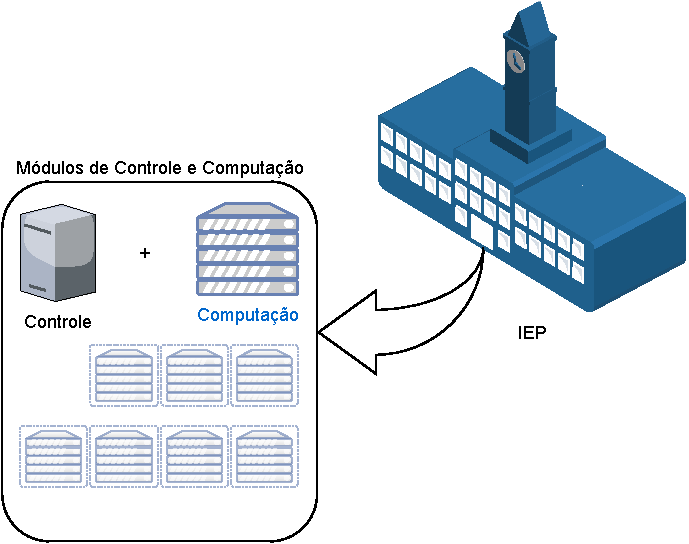
\includegraphics[scale=.8]{images/IEPNosModulos-v2.drawio.pdf}
	\caption[Composição dos nós da nuvem nas Instituições de Ensino e Pesquisa.]{Composição dos nós da nuvem nas Instituições de Ensino e Pesquisa.} 
	\label{fig:IEPNosModulos}
\end{figure}

O papel do módulo de controle é o de gerenciar todos os elementos do nó da nuvem alocados em uma IEP. Este módulo atua como ponto de agregação para as interconexões entre os módulos de computação, equipamentos de armazenamento e conexões, via rede, com o restante da infraestrutura da instituição hospedeira, possibilitando, assim, o compartilhamento dos recursos de hardware com os demais membros da nuvem federada. O módulo de computação oferece o poder de processamento do nó, adicionando \emph{cores} e espaço de armazenamento ao \emph{storage} localizado no módulo de controle.

A partir da classificação apresentada na Seção \ref{sec:instfederadas}, Tabelas \ref{tab:instpar} e \ref{tab:noporinst}, fica posto que as IEPs poderão dispor de até oito módulos de computação, dependendo do nível no qual forem enquadradas, compondo assim um nó da nuvem. Destaca-se que, no modelo proposto para a solução, um módulo de computação não pode ser disposto sem a existência de um módulo de controle. Assim, a menor configuração de um nó da nuvem é composta por, pelo menos, dois módulos, um de controle e outro de computação. Na hipótese de um crescimento do poder de processamento em uma instituição, excedendo a composição máxima de um nó, ou seja, 8 módulos de computação, essa instituição deverá prover a instalação de um segundo nó.

Com relação às especificações técnicas de processamento, armazenamento e conexões de rede, na Tabela \ref{tab:modulosespec} é apresentada uma possibilidade de configuração para os módulos de controle e computação. Essa configuração é a considerada no restante deste trabalho.

\begin{table}[H]
    \centering
    \caption{Especificações de hardware dos módulos de controle e computação.}
    \label{tab:modulosespec}
    \begin{tabular}{@{}lrrrl@{}}
        \toprule
        \multicolumn{1}{c}{\textbf{Módulo}} &
        \multicolumn{1}{c}{\textit{\textbf{Cores}}} &
        \multicolumn{1}{c}{\textbf{Memória RAM (GB)}} &
        \multicolumn{1}{c}{\textbf{Interfaces de Rede}} &
        \multicolumn{1}{c}{\textbf{Armazenamento}} \\ \midrule
        Controle   & 16 & 256 & 24 & 10TB* \\
                   &    &     &    &               \\
        Computação & 64 & 512 & 2  & 1TB** \\ \bottomrule
    \end{tabular}
    \caption*{*~ Quantidade de armazenamento inicialmente disponível no módulo de controle.\\ ** Quantidade de armazenamento adicionada por cada módulo de computação.}
\end{table}
  
O módulo de controle não necessita de recursos dedicados às tarefas de computação devido ao seu papel de gerenciamento dentro da solução. Os recursos de armazenamento, provenientes das adições de novos módulos de computação, são recepcionados na estrutura de \emph{storage} oferecida pelo módulo de controle.


% Aqui descrever a configuração de um nó. Imagino caixinha tipo plug-and-play, com recursos de rede e tudo. Até imagino que existam dois tipos de caixinha, um com switch e outro não. Bom, talvez um terceiro tipo, com storage. Não, dois tipos: um com switch e storage e outro só processamento. Caixinha basic e caixinha HPC. Imagino, talvez, a proporção de uma caixinha basic para até 8 caixinhas HPC.

% Para definição das especificações técnicas do nó de computação, o qual pode ser uma única máquina ou um conjunto de equipamentos, que será disponibilizado para as Instituições de Ensino e Pesquisa, foram levadas em consideração tecnologias atuais de mercado, com base em produtos ofertados pelos principais fabricantes de hardware.

\section{Interligação entre Nós}\label{sec:rede}

A interligação entre os nós que compõe a infraestrutura de nuvem federada merece destaque em função de características  necessárias para que seu funcionamento esteja de acordo com as expectativas dos usuários.

Por ser um infraestrutura geograficamente distribuída, com pontos de conexão localizados em diferentes cidades do estado do Rio Grande do Sul, a existência de uma rede de comunicação de dados estável e suficiente para o desempenho das atividades, as quais se propõe a nuvem federada, é de suma importância para a concretização do projeto. Tal rede deve ser capaz de prover comunicação a todos os nós da nuvem, alocados nas IEPs do estado.

Atualmente, as instituições candidatas a membro da federação de nuvem proposta, estão conectadas por meio da infraestrutura de comunicação ofertada pela Rede Tchê. Tal estrutura já permite, de modo imediato, a troca de informações entre as IEPs do estado do Rio Grande do Sul.

Por apresentar uma capilaridade bem distribuída entre as instituições que, eventualmente, se credenciem a fazer parte da infraestrutura de nuvem federada, a Rede Tchê é uma opção de conexão a ser considerada, com o objetivo de oferecer as capacidades de interconexão exigidas pelos nós da nuvem. A Rede Tchê é uma infraestrutura de rede de computadores que interliga IEPs, no caso, Universidades, Institutos Federais e Centros de Pesquisa, no estado do Rio Grande do Sul. Hoje, todas as instituições se conectam ao nó da Rede Tchê localizado na cidade de Porto Alegre, o qual se configura como a porta de entrada da rede e ponto de conexão à Internet, e com o resto do país, por meio do Ponto de Presença da RNP (Rede Nacional de Ensino e Pesquisa) no Rio Grande do Sul. Isso possibilita que as instituições conectadas desenvolvam vários projetos por meio da infraestrutura disponibilizada pela Rede Tchê e suas abrangências locais.

Uma alternativa à Rede Tchê seria a criação de uma rede de comunicação, entre as IEPs, com topologia em anel duplo, exclusiva para o tráfego de informações pertinentes ao usuários da nuvem federada. A topologia de rede em anel duplo permite que o tráfego flua em dois sentidos diferentes, permitindo um melhor aproveitamento da banda de rede disponível e garantindo um bom nível de redundância para a estrutura. Tal rede alternativa proveria acesso por meio de \emph{links} dedicados entre cada localidade na qual se encontre nós da infraestrutura de nuvem. Para a concretização de um projeto de rede como o citado anteriormente, seriam necessários investimentos financeiros por parte da instituições, além dos recursos que já seriam empregados para disposição dos nós a serem integrados à nuvem federada. O uso de uma rede alternativa pode configurar um ambiente, de certa forma, independente no que diz respeito a eventuais restrições impostas por empresas operadoras de serviços de telecomunicações. Porém, há de se considerar que a construção de uma rede alternativa implica em altos custos tanto de implantação quanto de manutenção, que poderiam inviabilizar financeiramente a concretização de um projeto de nuvem federada.

% \textcolor{blue}{Apresentar a rede tche como a rede que já existe e que poderia ser utilizada de forma imediata. Então descrever a rede tche. Depois, comentar que outras possibilidades poderiam ser adotadas, e então descrever quais requisitos e qual tipo de topologia poderia ser adotada.}\textcolor{red}{A vantagem de descrever desta forma é que justifica a avaliaçção usando a capilaridade da rede tche e a realização de novos casos de estudo com alternativas à ela.}

\section{Conclusão do Capítulo}\label{sec:concap}

Neste Capítulo foram apresentadas as condições para que uma IEP possa se credenciar como membro de uma infraestrutura de nuvem federada, de acordo com o modelo proposto por este trabalho.

A partir de critérios estabelecidos, foi possível definir um enquadramento para as instituições, estabelecendo-se níveis de classificação que serviram como base para definição de quantidades de módulos de recursos computacionais que devem ser dispostos pelas IEPs, como parte do acordo de participação no ambiente de nuvem federada.

% Com uma capilaridade bem distribuída entre as instituições que, eventualmente, se credenciem a fazer parte da infraestrutura de nuvem federada, a Rede Tchê é uma opção de conexão a ser considerada, com o objetivo de oferecer as capacidades de interconexão exigidas pelos nós da nuvem. A Rede Tchê é uma infraestrutura de rede de computadores que interliga IEPs, no caso, Universidades, Institutos Federais e Centros de Pesquisa, no estado do Rio Grande do Sul. Atualmente, todas as instituições se conectam ao nó da Rede Tchê localizado em Porto Alegre, o qual é se configura como a porta de entrada e ponto de conexão à Internet, e com o resto do país, por meio do Ponto de Presença da RNP no Rio Grande do Sul. Isso possibilita que as instituições conectadas desenvolvam vários projetos por meio da infraestrutura disponibilizada pela Rede Tchê e suas abrangências locais.

% Atualmente, só é possível conectar-se diretamente a Porto Alegre. O nodo de Porto Alegre é a porta de entrada da rede no Estado e ponto de conexão com o resto do país através do Ponto de Presença do Rio Grande do Sul. Neste nodo também existe uma conexão com o Ponto de Troca de Tráfego Internet no Rio Grande do Sul, o RSiX, onde estão conectados vários backbones comis e acadêmicos. As instituições podem estabelecer conexão por meio de linhas dedicadas, próprias ou alugadas de diversas teles que hoje possuem equipamentos no PoP-RS. Também é possivel a conexão utilizando enlaces via fibra óptica, rádio, ADSL ou cable-modem providos pelas teles locais. As várias instituições conectadas desenvolvem inúmeros projetos através da estrutura disponibilizada pela rede nas suas regiões de abrangência no estado.


\section{Elaboração da Estratégia de Escalonamento e Identificação de Limites da Estrutura}

- Propor uma estratégia de escalonamento mais elaborada, considerando alguns critérios (temos que ver estes critérios)\\
- Reavaliar os custos\\



%\chapter{Desenvolvimento}

\chapter{Desempenho na Nuvem Federada}

\noindent- simulações\\
- mapeamento quadrupla - google\\
- mapeamento dos traces do google para quadruplas (quais colunas devem ser selecionadas para representar a estrutura de quádrupla)\\
- como "executar" a quádrupla dentro do simulador (penso que deva ser algo como, na classe que faz a leitura dos arquivos do Google, ler os dados somente das colunas mapeadas que refletem o formato e os dados que interessam para as equivalência com as quádruplas)\\
- 

Nesse capítulo avaliar, com o Simulador, o desempenho da rede federada considerando a topologia especificada. Avaliar o desempenho/custo considerando o crescimento da demanda. Nesse momento, a estratégia básica é, a aplicação é lançada no sitio X e, então, priorizada sua execução em X mesmo. Se não der, exporta a aplicação. \textcolor{blue}{Pergunta: existe como realizar escalonamentos no simulador que considerem a data de término da aplicação? Caso tenha, poderemos pensar em como explorar.}

\begin{figure}[H]
	\centering 
	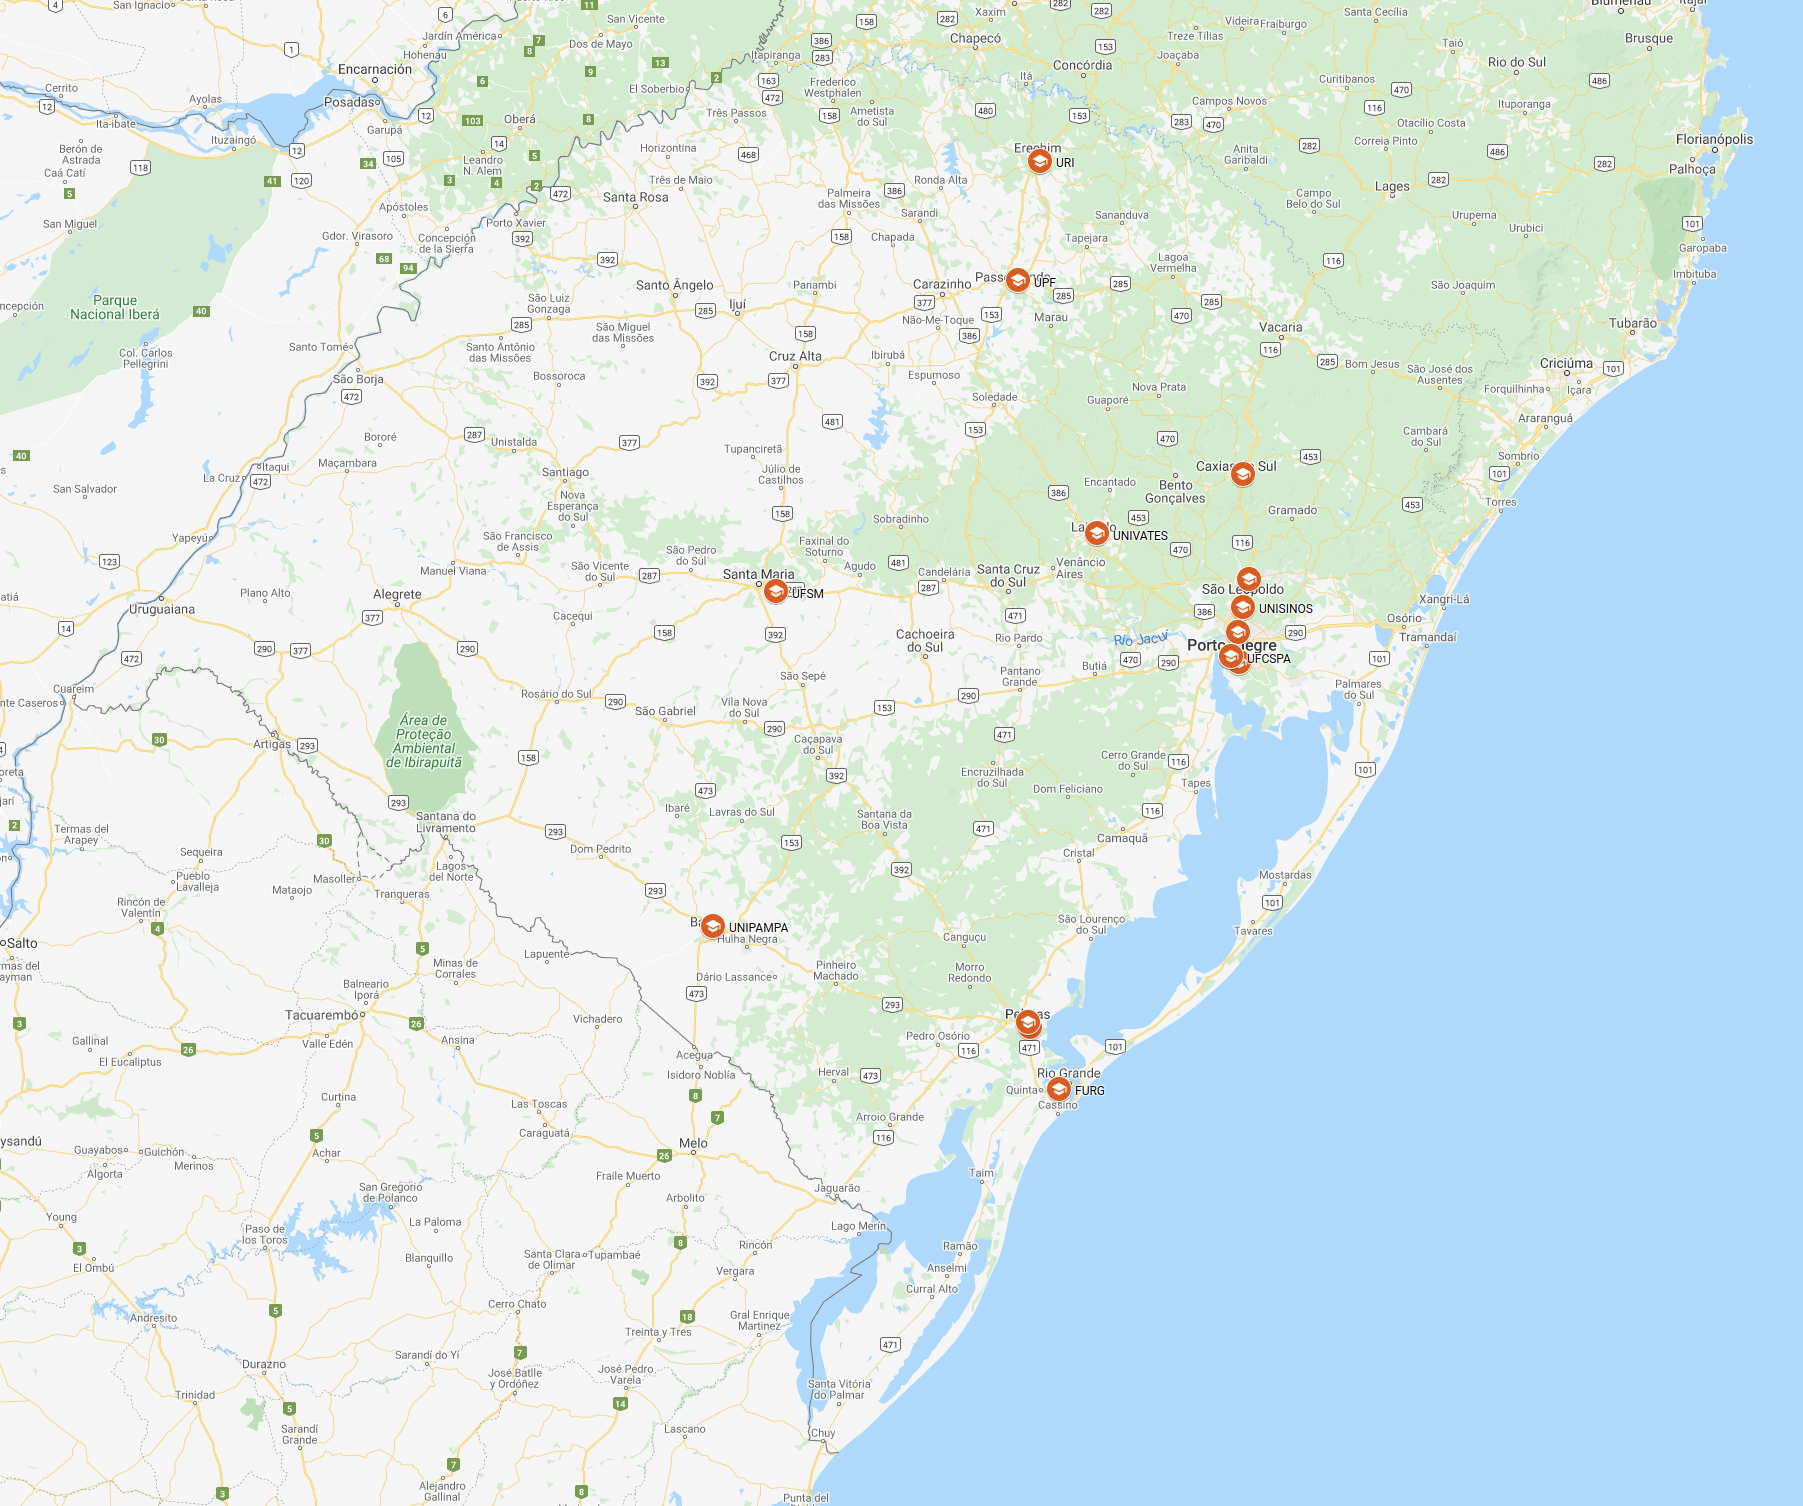
\includegraphics[scale=.25]{images/IEP.png}
	\caption[Distribuição geográfica das IEPs no Estado do Rio Grande do Sul.]{Distribuição geográfica das IEPs no Estado do Rio Grande do Sul.} 
	\label{fig:IEP}
\end{figure}

\section{Caracterização das Aplicações}\label{sec:caracaplic}

% Anotações:
%   \begin{itemize}
%       \item Apresentar extensões para o CloudSim é uma contribuição
%       \item Queremos contabilizar o custo de uma infraestrutura em nuvem:
%         \begin{itemize}
%             \item Considerando um trabalho atendido somente com os recursos locais
%             \item Considerando o atendimento com o cluster "federado"
%             \item Considerando o cloud bursting
%         \end{itemize}
%         \item Os cenários devem ser simulados de forma a permitir contabilizar estes custos.
%   \end{itemize}

% \textbf{Passo 1: Implantação do ambiente de nuvem}\\
% - identificar o "nó computacional" base (vai ser definido da cabeça)\\
% - identificar as instituições parceiras\\
% - identificar quantos nós cada instituição tem\\
% - interligar as instituições\\

% \textbf{Passo 2: avaliação preliminar}\\
% - gerar carga a partir das instituições parceiras\\
% -- em função de traço sintético\\
% - utilizar uma estratégia de distribuição da carga "simples" (algo que considere apenas disponibilidade de recursos nas outras instituições)\\
% - avaliar o comportamento a medida em que escala o aumento da demanda de processamento por instituição ou globalmente\\
% - individualizar o "custo" de uso da nuvem pelas instituições\\
% -- contabilizar o custo de ociosidade\\

% \textbf{Passo 3: Elaboração de estratégia de escalonamento e identificação dos limites da estrutura}\\
% - Propor uma estratégia de escalonamento mais elaborada, considerando alguns critérios (temos que ver estes critérios)\\
% - Reavaliar os custos\\

% 

% \section{Implantação do Ambiente de Nuvem}

% - identificar o "nó computacional" base (vai ser definido da cabeça)\\
% - identificar as instituições parceiras\\
% - identificar quantos nós cada instituição tem\\
% - interligar as instituições\\

% Para definição das especificações técnicas do nó de computação padrão, o qual pode ser uma única máquina ou um conjunto de equipamentos, que será disponibilizado para as Instituições de Ensino e Pesquisa, foram levadas em consideração tecnologias atuais de mercado, com base em produtos ofertados pelos principais fabricantes de hardware.

% Entende-se por nó de computação padrão a infraestrutura física, em termos de computadores servidores, que será ofertada pela Instituição para uso local e pelas demais Instituições participantes da solução de nuvem computacional em nível estadual.

% Com base no Mapa de Investimentos do \textdecor[GoogleYellow!35, draw=GoogleYellow!35]{CNPq}\ups{adicionar à lista de siglas} (Conselho Nacional de Desenvolvimento Científico e Tecnológico), disponível na Internet em \url{http://efomento.cnpq.br/efomento/distribuicaoGeografica/distribuicaoGeografica.do?metodo=apresentar}\improve{transformar em referência formal}, sob a modalidade de "Apoio a Projetos de Pesquisa", foram selecionadas 15 instituições, contemplado Universidades e Institutos Federais, com maior percentual de participação em Projetos de Pesquisa no Estado do RS.

% \begin{table}[H]
%   \centering
%   \caption{Instituições Parceiras}
%   \label{tab:my-table}
%   \resizebox{\textwidth}{!}{%
%   \begin{tabular}{@{}|l|l|l|@{}}
%   \toprule
%   Instituição                                                        & Sigla      & \# projetos \\ \midrule
%   Universidade Federal do Rio Grande do Sul                          & UFRGS      & 280         \\ \midrule
%   Universidade Federal de Santa Maria                                & UFSM       & 108         \\ \midrule
%   Universidade Federal de Pelotas                                    & UFPEL      & 88          \\ \midrule
%   Universidade Federal do Rio Grande                                 & FURG       & 60          \\ \midrule
%   Universidade do Vale do Rio do Sinos                               & UNISINOS   & 57          \\ \midrule
%   Pontifícia Universidade Católica do Rio Grande do Sul              & PUCRS      & 44          \\ \midrule
%   Universidade de Caxias do Sul                                      & UCS        & 28          \\ \midrule
%   Universidade Federal do Pampa                                      & UNIPAMPA   & 21          \\ \midrule
%   Fundação Universidade Federal de Ciências da Saúde de Porto Alegre & UFCSPA     & 13          \\ \midrule
%   Universidade do Vale do Taquari                                    & UNIVATES   & 13          \\ \midrule
%   Universidade de Passo Fundo                                        & UPF        & 10          \\ \midrule
%   Universidade Feevale                                               & FEEVALE    & 10          \\ \midrule
%   Universidade La Salle                                              & UNILASALLE & 9           \\ \midrule
%   Universidade Regional Integrada do Alto Uruguai e das Missões      & URI        & 9           \\ \midrule
%   Instituto Federal Sul-rio-grandense                                & IFSul      & 8           \\ \bottomrule
%   \end{tabular}%
%   }
%   \end{table}

Como critério para definir a quantidade de nós de computação que cada instituição teria, foi utilizada a seguinte condição:

% \begin{table}[H]
%   \centering
%   \caption{Nós por Instituição}
%   \label{tab:noporinst}
%   \begin{tabular}{@{}l|l@{}}
%   \toprule
%   \# projetos & \# nós \\ \midrule
%   1 a 10      & 1      \\ \midrule
%   11 a 50     & 2      \\ \midrule
%   51 a 100    & 4      \\ \midrule
%   100+        & 8      \\ \bottomrule
%   \end{tabular}%
%   \end{table}

\section{Avaliação Preliminar}

- gerar carga a partir das instituições parceiras\\
-- em função de traço sintético\\
- utilizar uma estratégia de distribuição da carga "simples" (algo que considere apenas disponibilidade de recursos nas outras instituições)\\
- avaliar o comportamento a medida em que escala o aumento da demanda de processamento por instituição ou globalmente\\
- individualizar o "custo" de uso da nuvem pelas instituições\\
-- contabilizar o custo de ociosidade\\

\section{Mapeamento googleclusterdata --> quádrupla}

aqui vamos escrever... 

ok, vamos tentar.

\chapter{Introdução de Cloud Bursting}

No capítulo anterior, a simulação foi até o ponto em que a demanda dos usuários suplantou a oferta de recursos, aumentando o tempo de espera dos usuários. Uma alternativa é o incremento dos recursos, implicando em gastos. Outra é utilizar cloud bursting. Nesse capítulo discutir os custos associados ao cloud bursting. É possível que uma estratégia de escalonamento deva ser realizada. Imagino que o escalonamento opere da seguinte forma: tenta lançar local, se não deu, tenta lançar em um outro sítio, se não deu, dispara na pública. Em execução, a medida em que um sitio se torna ocioso, busca para executar o que está na nuvem.

\section{Definição de Cloud Bursting}

Cloud bursting pode ser definido como a utilização temporária de recursos de nuvens computacionais por meio de infraestruturas de nuvens híbridas \cite{Jigsaw2021}. Neste modelo de implantação, as aplicações que são executadas em ambientes locais, como nuvens privadas, são repassadas, geralmente uma parte, para nuvens privadas, com o objetivo de evitar a interrupção dos serviços.

De modo geral, as organizações reservam a opção de cloud bursting para aplicações que tendem a gerar picos de demanda e grandes flutuações na utilização de recursos computacionais. No entanto, aplicações muito complexas ou que dependam de recursos específicos de computação não costumam ser boas candidatas para a execução explodida em uma nuvem pública \cite{NetApp2020}.

A utilização de nuvens públicas, como complemento para os recursos locais de computação, pode se tornar uma opção mais prática às organizações que já operam seus próprios sistemas computacionais \emph{in-house}. Vantagens como escalabilidade, com o uso de escalonamento horizontal, na qual picos esporádicos de cargas de trabalho podem ser tratadas de forma mais eficaz; a utilização de recursos, na qual o nível de provisionamento pode ser ajustado para a carga de trabalho em níveis normais de uso; e a segurança que permite que uma política multinuvem possa ser aplicada, principalmente, devido à adoção de nuvens públicas. Em ambientes que fazem uso de cloud bursting, os dados confidenciais poderiam ser mantidos e tratados no ambiente privado (nuvem privada) ao passo que cargas de trabalho menos sensíveis à políticas de segurança poderiam ser transferidas para nuvens públicas sem comprometimento da confidencialidade dos dados \cite{leeCloudBurstingScheduler2017}.

% No entanto, como muitas organizações já operam seus próprios sistemas computacionais, o uso dinâmico de nuvens públicas além de recursos próprios (cloud bursting) é uma opção mais prática. Defendemos o cloud bursting com três vantagens: (1) escalabilidade (escalonamento horizontal: picos esporádicos de carga de trabalho podem ser tratados de forma eficaz, (2) utilização de recursos: o nível de provisionamento de recursos pode ser definido para a carga de trabalho média/normal e (3) segurança: a a política de segurança multinuvem pode ser aplicada. A segurança é uma grande preocupação com a adoção da nuvem pública. Com a explosão da nuvem, os dados confidenciais podem ser mantidos e processados no sistema privado, e cargas de trabalho menos sensíveis à segurança podem ser transferidas para a nuvem pública. 



% \cite{Microsoft2022}



\section{Determinar Vantagens e Desvantagens (financeiras) de Realizar Cloud Bursting}

- Agora se apresenta a necessidade de "crescer" a infraestrutura: aumentar a quantidade de recursos ou alugar uma nuvem pública\\
- Reaplicar a estratégia do Passo 3 neste novo contexto\\
- Reavaliar os custos\\

\chapter{Impacto nos Custos}

Aqui relacionar vantagens e desvantagens das soluções: incrementar a nuvem, realizar bursting.

%   Bla blabla blablabla bla.  Bla blabla blablabla bla.  Bla blabla
%   blablabla bla.  Bla blabla blablabla bla.  Bla blabla blablabla bla.
%   Bla blabla blablabla bla.  Bla blabla blablabla bla.  Bla blabla
%   blablabla bla.  Bla blabla blablabla bla.  Bla blabla blablabla bla.
%   Bla blabla blablabla bla.  Bla blabla blablabla bla.  Bla blabla
%   blablabla bla.  Bla blabla blablabla bla.  Bla blabla blablabla bla.
%   Bla blabla blablabla bla.  Bla blabla blablabla bla.  Bla blabla
%   blablabla bla.  Bla blabla blablabla bla.  Bla blabla blablabla bla.
%   Bla blabla blablabla bla~\ref{tabela2}.

% \begin{table}
% \begin{center}
% \caption{Nome da Tabela}\label{tabela2}
% \begin{tabular}{p{4cm}p{5cm}p{6cm}}
% \hline
% Blabla & Blabla & Blablabla\\
% \hline
% {\small Bla} & {\small Blabla} & {\small\em Bla blabla blablabla blabla
%   blablabla blabla blablabla.}\\
% {\small Bla} & {\small Blabla} & {\small\em Bla blabla blablabla blabla
%   blablabla blabla blablabla.}\\
% {\small Bla} & {\small Blabla} & {\small\em Bla blabla blablabla blabla
%   blablabla blabla blablabla.}\\
% {\small Bla} & {\small Blabla} & {\small\em Bla blabla blablabla blabla
%   blablabla blabla blablabla.}\\
% {\small Bla} & {\small Blabla} & {\small\em Bla blabla blablabla blabla
%   blablabla blabla blablabla.}\\
% {\small Bla} & {\small Blabla} & {\small\em Bla blabla blablabla blabla
%   blablabla blabla blablabla. Conforme a figura~\ref{figura}}\\
% \hline
% \end{tabular}
% \end{center}
% \end{table}

% \begin{figure}[htbp]
%   \centering 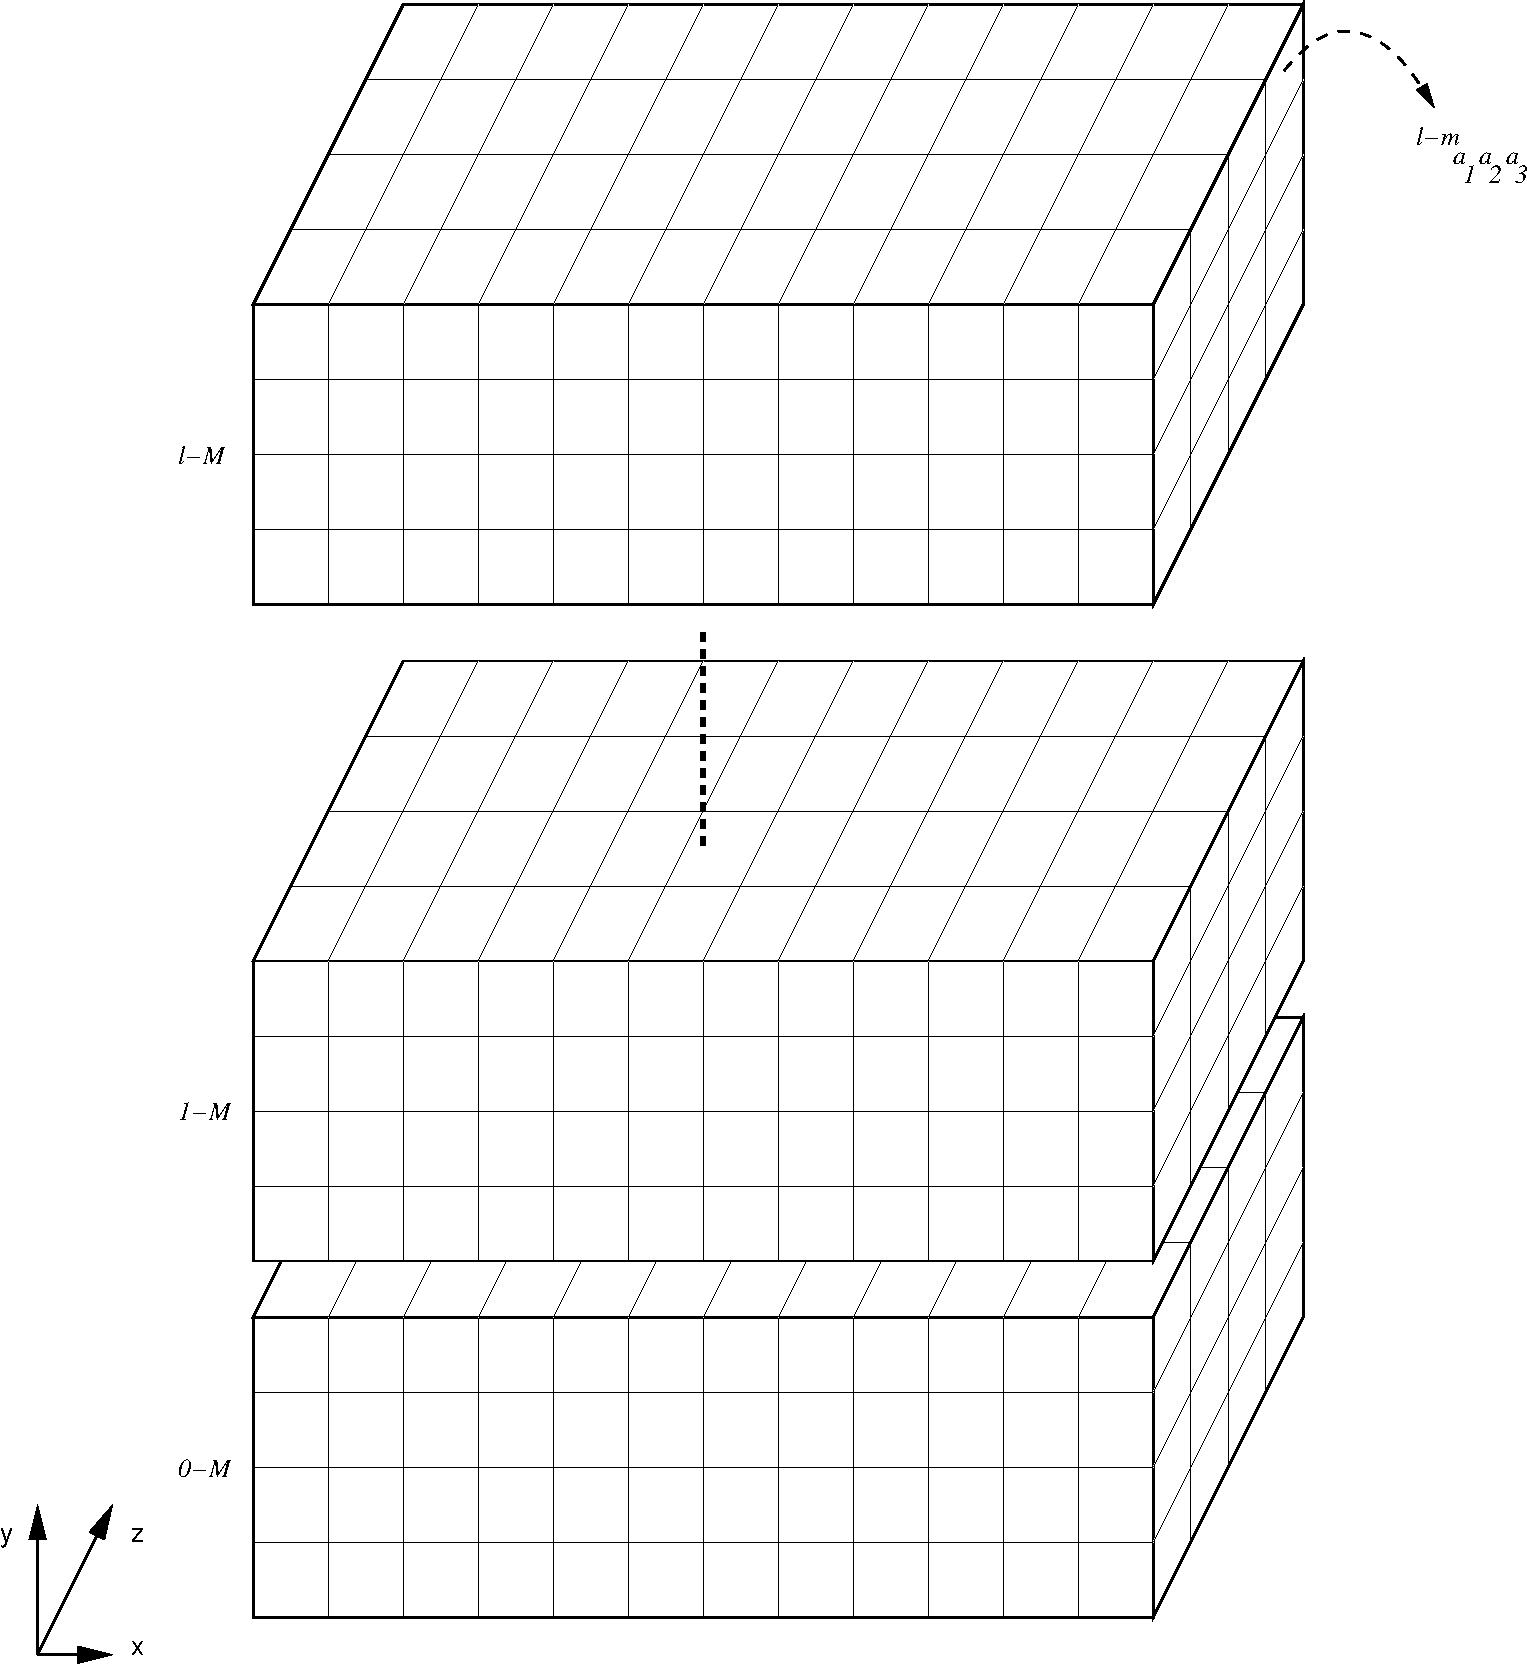
\includegraphics[scale=.4]{figura}
% \caption{Nome da figura} 
% \label{figura}
% \end{figure}


\chapter{Conclusão}



% Bibliografia http://liinwww.ira.uka.de/bibliography/index.html um
% site que cataloga no formato bibtex a bibliografia em computacao
% \bibliography{nomedoarquivo.bib} (sem extensao)
% \bibliographystyle{formato.bst} (sem extensao)

\bibliographystyle{abnt}
\bibliography{madsantos} 

% % Apêndices (Opcional) - Material produzido pelo autor
% \apendices
% \chapter{Um Apêndice}

% % Anexos (Opcional) - Material produzido por outro
% \anexos
% \chapter{Um Anexo}



% \chapter{Outro Anexo}



% Faz a capa do CDROM
% \makecover

\end{document}